\chapter[Introduction]{Introduction}
\label{sec:1_Introduction}


\chaptermark{Introduction}

%\chapterauthor{Hein Mannaerts}

Welcome to chapter 1 on "Overview of Quantum Communications".
In this chapter, we will give you an overview of how communication has evolved over the many thousands of years, 
then we will tell you about sending signals between parties of a network.
We will tell you the differences and similarities between digital and analog signals.
We will introduce the fundamental building block of modern communication, the \emph{bit}.
We will move on to quantum communication and explain why you should care about it, what new capabilities that it brings to the table, and what the new challenges are that face us in designing quantum communication systems. 
We will move on to the disruptive nature of quantum technologies and quantum communication in particular.
We will conclude this chapter by giving you an overview of the entire module, what the prerequisites are, what you will learn, and the outcomes of the module.


\section{History of Communication}

Methods of communication advance in order to accommodate a growing society while new technological advances allow society to grow and expand.

Humans are social creatures by nature.
Effective communication has been crucial to our survival;
in particular, it has been very important in sharing information about potential new sources of food and danger.
We communicated by gathering around the fire and talking to each other as illustrated in Fig.~\ref{fig:1-1_communication}.
Over many thousands of years, the methods of communication have evolved to become more efficient and longer ranging until we have finally reached our modern age where nearly every device that we have in our possession, our phones, our TVs, our iPads, even our fridges are all connected to a massive internetwork, the Internet.
We can be separated by many thousands of kilometers, but when we communicate it almost feels as if we are all sharing the same fire like in the old times.
We have gone from local communication to a truly global communication.

\begin{figure}[h]
    \centering
    \includegraphics[width=0.6\textwidth]{lesson1/communication.eps}
    \caption[Evolution of communication]{Evolution of communication. At the start, all communicating parties had to be within earshot of each other to exchange information quickly and effectively. Today, thanks to the Internet, we can still do the same without worrying about the parties' locations.}
    \label{fig:1-1_communication}
\end{figure}

Let's see how such a massive transformation happened.
In the next couple of paragraphs, you're going to see some famous examples from history illustrating the many different ways in which we have communicated.
The most obvious way was to take your message, write it on a piece of paper and send the message directly.
A very famous example of this method was the Battle of Marathon in 490 BC, where the legend goes that a runner was sent from where the battle took place near the city of Marathon to Athens. \rdv{distance?}
But that is historically not true.
The Athenians were trying to gain support of the army from the city of Sparta, located around 225 kilometers away.
The Athenians sent a runner carrying their message to Sparta.
And that journey, believe it or not, took a little less than a day.

Another method of sending a message directly was using birds such as homing pigeons.
There are pigeons that were specially trained to always return to their homes or their coops. People used to put the pigeons in cages when traveling somewhere. Whenever they needed to send a message back home, they would take a little piece of parchment paper, write the message down, attach it to the pigeon's leg, and let the pigeon go. The pigeon would automatically fly back and deliver the message.
The range of these birds was around a very impressive 1600 kilometers.
The average speed was around 95 kilometers per hour.
The top speed of some very athletic pigeons was upwards of 160 kilometers per hour.

Our final example of sending messages directly is the Pony Express.
The Pony Express was a company set up in the mid-nineteenth century in the United States to connect the east and west coasts.
If you were on the east coast and you wanted to send a letter to somebody on the west coast, you went to this company, and then they would send a horse and rider who would deliver your message.
The messenger would ride the horse to a relay station on the way, change to a fresh horse and continue with your message onwards to the next relay station.
Believe it or not, the entire journey of 4,000 kilometers took approximately 10 days.
In the context of communication speeds at the time, this was very, very fast.
Not only could you send letters, but you could also send some small parcels.
The Pony Express was the very early Amazon!
But despite the company's successful system, it only existed for one year; it was an early victim of the advance of technology, because it was created just as the method of communication was changing from direct transmission to electrical telegraphy.

But before we get to this revolution in communication technology, let's talk about these different ways of sending a message.
Sending a message directly in the form of a written letter is generally \textit{\textbf{slow}} and suffers from \textit{\textbf{reliability issues}}.
You may lose your pigeon, or your runner may become exhausted and just give up the task.
If this happens you have to find another pigeon or runner and resend the message, provided that you are even aware that the message has not been delivered yet.

An alternative to direct transmission was \textit{\textbf{optical telegraphy}}.
This is an old but ingenious method where the sender and the receiver share some pre-agreed signals.
The sender uses some optical means in order to generate these signals such that the receiver can see them.
A very good example is the Great Wall of China which was designed and built to protect the northern border of the Chinese Empire.
Due to its vast length, it was crucial to devise a communication system that could quickly relay messages between the guard towers located along the Wall.
Whenever the enemy tried to attack the Wall, the nearest guard tower would light its fire. This fire was then observed from the neighboring guard towers, which were approximately 2.5-5 kilometers apart.
Then they would light their fires.
Then their neighbors would see that and light their fires.
This is how the message spread across large portions of the Wall very quickly.
One drawback was that the \textit{\textbf{expressibility}} of this communication method was limited.
Only certain messages could be sent.
For example, the enemy is here or it's not, the fire is burning or it's not.
One could develop this method a little bit further by introducing a second fire at each guard house.
When one fire is burning, the enemy is there but in small numbers.
When two fires are burning, the enemy is there in large numbers.
Despite the limited expressiveness of this communication method, this system was very efficient and served well in protecting the Wall.

\begin{figure}[t]
    \centering
    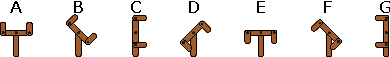
\includegraphics[width=0.7\textwidth]{lesson1/1-1_napoleon.pdf}
    \caption[Napoleon's semaphore]{Napoleon's semaphore encodings for the first five letters of the alphabet.}
    \label{fig:1-1_napoleon}
\end{figure}

Our last example of optical telegraphy is known as \textit{\textbf{Napoleon's semaphore}}.
This system was a lot more expressive than the signalling system of the Great Wall.
It worked on the basis of crane arms which could be arranged at certain angles.
An operator controlled levers and pulleys in order to arrange the arms at various angles. Each configuration of the arms carried its own meaning.
The leftmost arm configuration in Fig.~\ref{fig:1-1_napoleon} corresponds to the letter ``A".
A network of semaphores, each located around 10 kilometers apart, spanned all of France.
It was possible to send a message from Paris all the way to Venice, a distance of 1100 kilometers, in as little as few hours.
The record time of sending a message between Paris and Strasbourg in the east of France, was an astounding 1 hour.
This would have been unthinkable using the direct communication discussed above.

But as you can imagine there were some drawbacks to this method, the biggest one being that you had to have \textit{\textbf{direct visual contact}} with your neighboring semaphore.
Therefore, the semaphore worked reliably only in good weather and during daytime.
In addition, even though you could express an arbitrary message using this method, it was \textit{\textbf{physically demanding}} to operate the crane arms.

This brings us finally to the reason why the Pony Express operated only for a single year: the advent of \textit{\textbf{electrical telegraphy}} and the invention of the \textit{\textbf{Morse code}} that used electric signals to transmit messages.
It worked by encoding the letters of the alphabet into a series of ``dots'' and ``dashes'' as seen in Fig~\ref{fig:1-1_morse}.
An operator used a telegraph key to close an electric circuit to produce a signal of desired length.
Closing the electric circuit for a short time produced a ``dot'' while keeping the circuit closed for a longer time produced a ``dash''.
If the length of a ``dot'' is one unit, then a ``dash'' has length of 3 units.
Parts of the same letter are separated by 1 unit.
Different letters are separated by a space of 3 units while different words are separated by 7 units.
A skilled operator could transmit up to 30 words per minute, which were decoded by an operator at a distant telegraph station and passed onto the intended recipient.
This communication method allowed for messages to be delivered across greater lengths, spanning continents within minutes, making direct communication such as the Pony Express or optical telegraphy such as Napoleon's semaphore obsolete.

\begin{figure}[t]
    \centering
    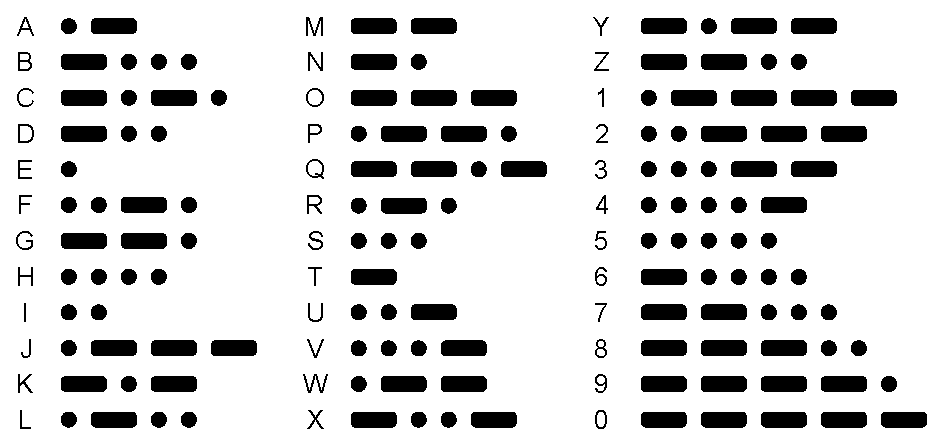
\includegraphics[width=0.8\textwidth]{lesson1/1-1_morse.eps}
    \caption[The Morse code]{The Morse code.}
    \label{fig:1-1_morse}
\end{figure}

Eventually, the electrical telegraph gave way to the \textit{\textbf{telephone}}, which implemented the dream of communication between humans using the human voice.
Early telephone connections were simple point to point.
As the demand for communicating via the telephone grew, it became clear the \textit{\textbf{all-to-all}} approach would not work.
Imagine a network of $N$ telephones where all of them are directly connected to each other as seen in Fig.~\ref{fig:1-1_telephone}.
Consider adding a new telephone to the network.
In order for the new user to be able to call any of the existing telephones on the network, we have to add $N$ physical connections to all of the existing telephones.
Adding yet another telephone would require another $N+1$ connections.
The all-to-all approach is intuitive but simply does not \textit{\textbf{scale}} with the size of the network.

\begin{figure}[h]
    \centering
    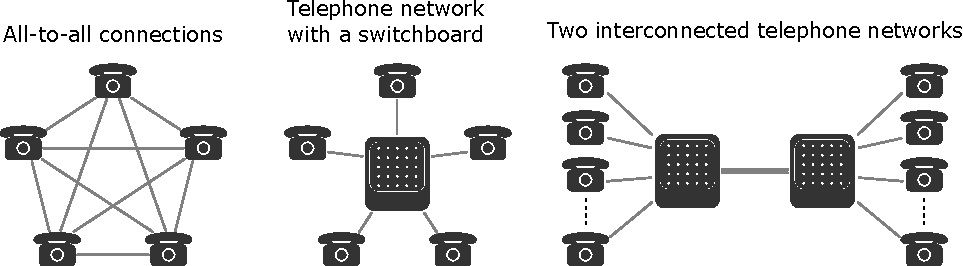
\includegraphics[width=\textwidth]{lesson1/1-1_rotary_telephone.pdf}
    \caption[Telephone networks]{Various topologies for telephone networks.}
    \label{fig:1-1_telephone}
\end{figure}

The solution came with the introduction of a \textit{\textbf{switchboard}}.
In order to call anybody on the network, each unit had to be connected only to the switchboard.
You first called the switchboard which would then connect you to the desired telephone unit.
With this approach, adding a new telephone to the network required adding a single connection to the switchboard, presenting a \textit{\textbf{constant scaling}}.
In other words, the effort of adding new users to the network did not increase with the size of the network.
Eventually, switchboards of different networks were interconnected together, allowing users from one network to call users on an entirely different network.

\begin{figure}[h]
    \centering
    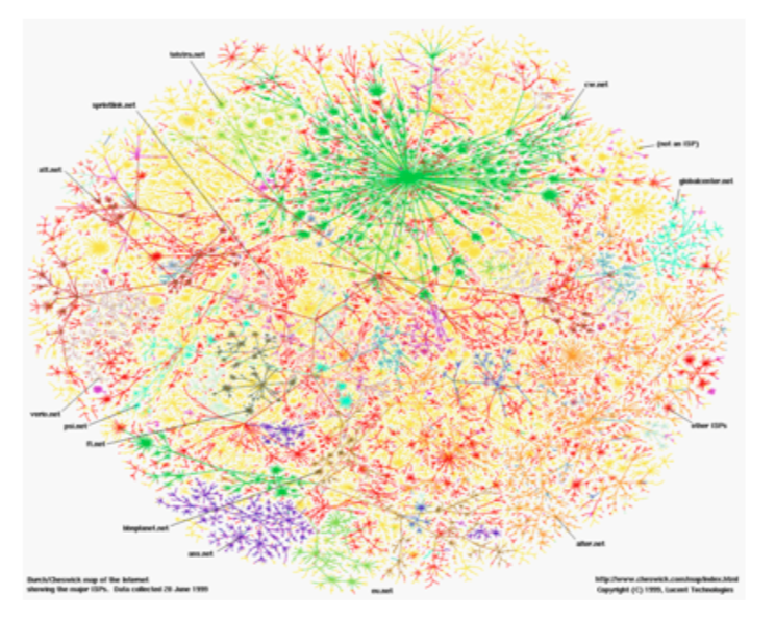
\includegraphics[width=0.8\textwidth]{lesson1/internetmap.eps}
    \caption[Map of the Internet.]{Map of the Internet.}
    \label{fig:1-1_internet}
\end{figure}

The Internet that our society has come to depend on so much works on the same principle.
It is not a single network but a \textit{\textbf{network of networks}}, allowing heterogeneous smaller networks to be interconnected.
Nowadays, a message sent from a laptop can be read by its recipient half-way around the world on their phone within seconds.
A broadcast stream of the FIFA World Cup Final can be enjoyed by millions around the world with minimal delay.
We can even start the air conditioning in some modern cars remotely without having to leave the comfort of our house.
Figure~\ref{fig:1-1_internet} depicts the closest thing to a ``map'' of the Internet that might be possible.
The dots do not represent individual hosts like computers or printers.
They represent entire networks!
The edges are the virtual connections between these networks.
This map of the Internet is not accurate due to its sheer size as well as as the fact that networks are constantly being added or removed.
Any ``map'' of the Internet that we might want to produce presents a monumental task, the results of which would quickly be outdated.
The only purpose such a map would serve would be to make us realize how far humanity's ability to communicate has come and make us wonder what the next step is in the evolution of communication.

% Today, we have the Internet which is a global spanning network of networks. Meaning that there are many different heterogeneous networks all connected to each other. So if you are using your phone, maybe you are connected to some telco tower which then relays the signal through the internet to wherever you wish. Also our computers are connected to modems via wi-fi, then these modems are connected to the Internet via ethernet cables. And basically everything is connected nowadays. We consume voice, and video entertainment, and news, and virtually we have access to any form of information that we wish to. And it's within a very short brief of time. So this image of internet is actually quite a simplification. In reality, what it looks like is more like this.

% So this rather confusing looking blob is a representation of the virtual connections between networks. So each of these little dots, they don't represent physical machines, they represent smaller networks. So you can see how complicated the routing in the Internet actually is. And this picture is about 20 years old. So nowadays probably it might look something a little bit even more impressive. So we have started with people gathering around campfires and sharing information, to having a truly global internet. But for us this is only where the journey begins. In this course, we will tell you what lies beyond the classical internet. What are the necessary tools to get there. And what are the challenges that face us.

\section{Analog to digital}

%Step 2: Analog to digital. 

The methods of communication described in the previous section were all very different from each other.
However, at a fundamental level they all followed the same basic principle depicted in Fig.~\ref{fig:1-2_communication}.
A sender \textit{\textbf{encodes}} her message into a form suitable for transmission.
The encoded message is then sent to the \textit{\textbf{decoder}}, which transforms the message back to a more easily readable form and passes it to the receiver.
To make this abstraction a little more concrete, let's consider the electrical telegraph as an example.
The sender brings her message to an operator who knows how to use the Morse key.
The operator uses the key to produce a series of dots and dashes, represented by short and long electrical signals which are transmitted to a distant telegraph station.
There another operator receives these electrical signals, decodes them and reproduces the original message for the receiver.

\begin{figure}[t]
    \centering
    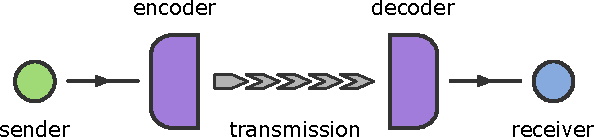
\includegraphics[width=0.7\textwidth]{lesson1/1-2_communication.pdf}
    \caption[Abstraction of communication]{Abstract representation of communication between a sender and a receiver.}
    \label{fig:1-2_communication}
\end{figure}

The immediate question that arises is finding some good ways of encoding the message.
The first method that we consider is encoding the message using an \textit{\textbf{analog}} signal.
Analog signals can admit a continuum of values.
We perceive the world around us as analog.
The loudness of sounds varies continuously from a quiet whisper to a loud music concert.
The temperature rises and falls in a continuous way as measured by our thermometers.
The three primary colors can be mixed together to produce a continuous spectrum of colors.
Humans have evolved to process these types of analog signals; therefore, it makes sense to try using analog signals to encode our messages.
The key is that analog signals can take on values from a continuous interval, representing the range of some quantity.
For example, the voltage of an electric circuit can vary continuously depending on the pressure of sound waves in the microphone of an old telephone.
Early AM radio signals and old TV broadcasting used continuous sinusoidal waves that required simple technology to produce and decode.

\begin{figure}[t]
    \centering
    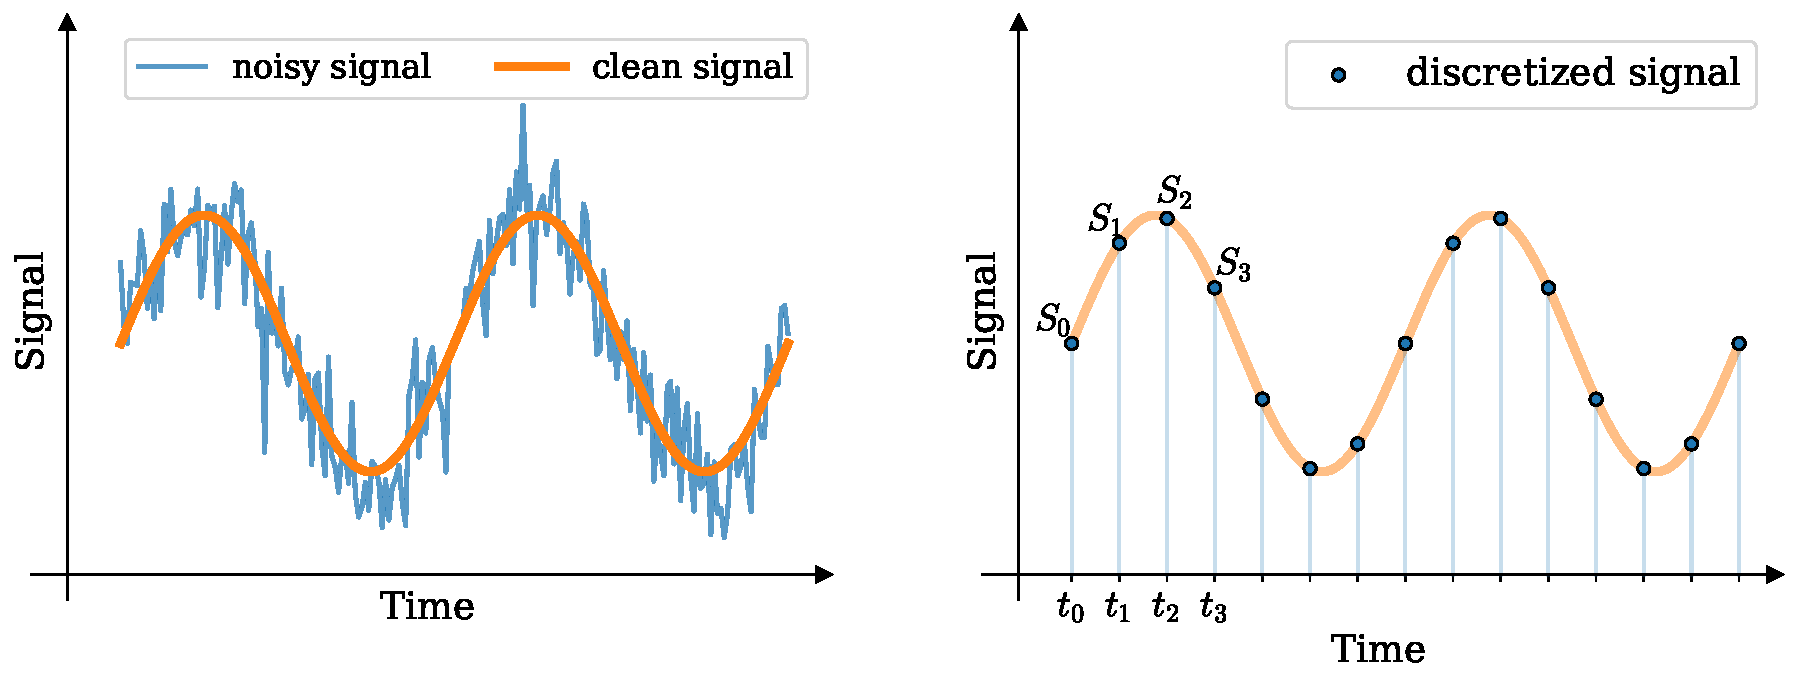
\includegraphics[width=\textwidth]{lesson1/1-2_signals.pdf}
    \caption[Continuous and discrete signals]{Analog signal subjected to noise on the left. The right figure shows how the analog signal can be discretized.}
    \label{fig:1-2_signals}
\end{figure}

One problem with analog signals is that they are \textit{\textbf{susceptible to noise}}.
Even small changes to the signal can alter the meaning of the transmitted message.
Due to this sensitivity to noise, analog signals are also difficult to copy.
Every time an analog signal gets copied, it degrades in quality due to both the noise as well as the finite accuracy the signal read out.

Figure~\ref{fig:1-2_signals} shows a clean analog sinusoidal signal in orange.
The blue jagged line represents the original signal affected by noise.
The noisy signal may have a meaning similar to the original noiseless message or may be quite different.

An alternative to analog signals is \textit{\textbf{digital}} signals.
Digital signals are very different from analog signals; they only use a discrete set of values to represent the message and encode it.
We can take the original analog signal, and try to encode it digitally.
A way to do this to \textit{\textbf{sample}} the analog signal at discrete time steps $t_0$, $t_1$, $t_2$, $t_3$ and so on, as shown on the right side of Fig.~\ref{fig:1-2_signals}.
The encoded digital signal is now a set of discrete values,
\begin{equation}
    S_0, S_1, S_2, S_3, \ldots,
\end{equation}
each of some finite accuracy.

The accuracy with which we can reproduce this analog signal depends on how often we look at and measure the signal, which is known as the \textit{\textbf{sampling rate}}.
For slowly varying signals, we don't have to sample that often, while still doing a pretty good job of encoding the analog signal accurately.
But for analog signals that vary quickly, we should sample with higher frequency.
Digital signals are less affected by noise and are therefore easier to copy.
Other advantages include the ease of producing digital signals and the ease of processing with digital logic.


\section{Bits as building blocks}

% Step three: Bits as building blocks. 

We have seen that digital signals can be more practical than analog signals when it comes to communication.
The question now is how do we represent these digital signals.
We saw an example of a digital system with Napoleon's semaphore.
Let's go back and consider it again.
In order to send a message, for example ``WAR IS OVER'', the arms have to be rearranged as shown in Fig.~\ref{fig:1-3_warisover}.

\begin{figure}[t]
    \centering
    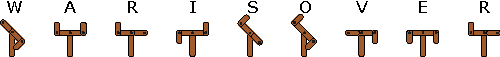
\includegraphics[width=0.8\textwidth]{lesson1/1-3_warisover.pdf}
    \caption[Message with Napoleon's semaphore]{Encoding a short message using Napoleon's semaphore.}
    \label{fig:1-3_warisover}
\end{figure}

What does it take to change the state of the semaphore?
Changing the state of the semaphore from ``A'' to ``R'' does not require that much effort.
All we have to do is change the state of one of the side arms and fold it onto the main arm.
On the other had, going from ``W'' to ``A'' requires changing the state of the main arm as well as the two side arms.
This change requires both physical effort as well as longer time.

\begin{figure}[t]
    \centering
    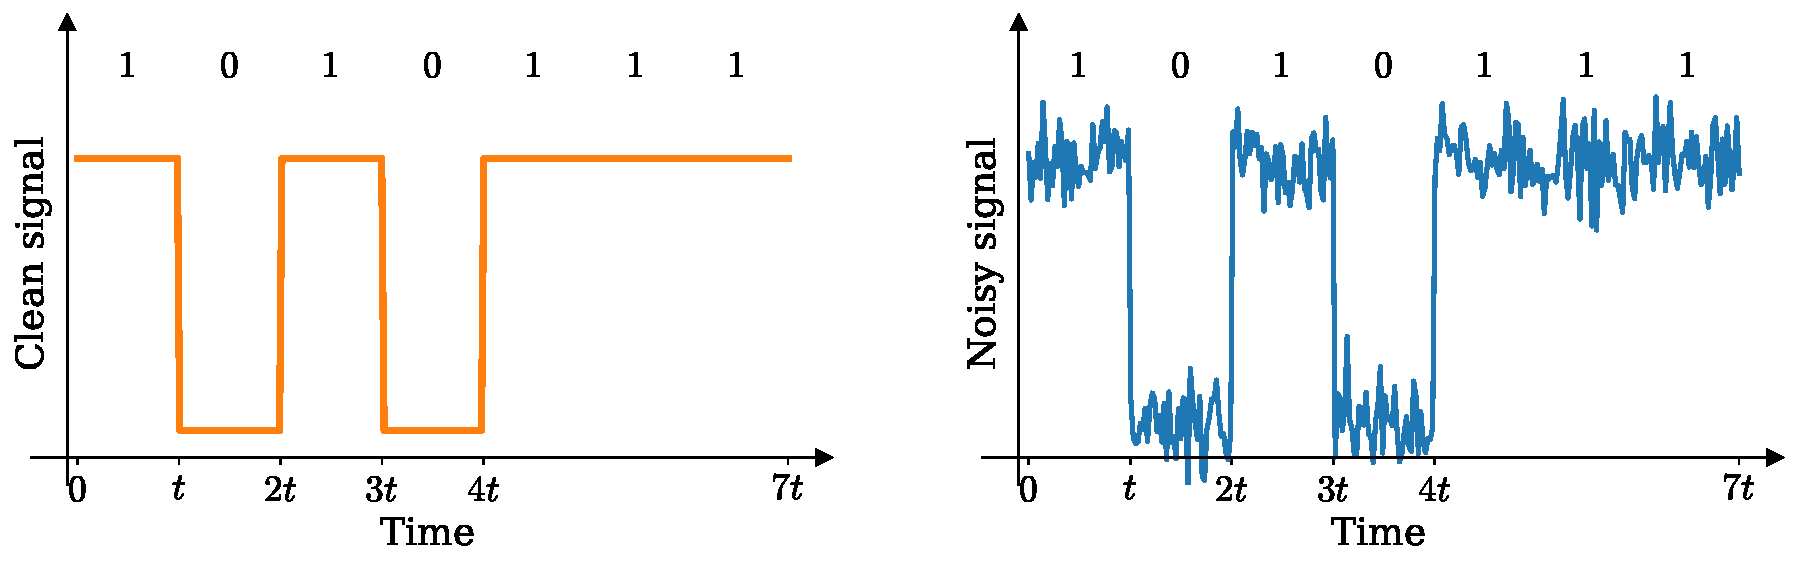
\includegraphics[width=\textwidth]{lesson1/1-3_morse_signal.pdf}
    \caption[Morse code signal]{Physical representation of the Morse code signal for the letter ``U''.}
    \label{fig:1-3_morse_signal}
\end{figure}

A good representation for digital signals should require as little effort and time as possible in order to change the state of the digital signal.
This suggests that having fewer internal states produces a better encoding for the message.
The Morse code is such an example, where we only have two internal states.
The letter ``U'' is encoded by two dots followed by a dash.
The physical signal that represents this encoding is shown in Fig. \ref{fig:1-3_morse_signal} on the right.
The signal is switched on for a short time to represent a dot and for a long time to represent the dash.
It is the presence or absence of a signal that conveys the information.
When you change from \emph{no signal} to \emph{signal}, or when the signal \emph{doesn't} change, this carries a small amount of information.

This unit of information is known as a \textit{\textbf{bit}}, which is short for \textit{\textbf{binary digit}}.
In classical computation and in digital communication, the bit is the basic unit of information.
It conveys the message of something being true or false, the signal being on or off.
Usually we write the two states of a bit as 0 or 1.
The signal on the left of Fig.~\ref{fig:1-3_morse_signal} encoding the letter ``U'' in Morse code can be written using bits as 1010111, where zeros and ones denote the state of the bit at different times.
The right side of Fig.~\ref{fig:1-3_morse_signal} shows how the clean signal looks after being affected by noise.
The different states of the bit can still be easily distinguished from each other, hence the meaning of the message can be read out without any ambiguity.
Digital signals are generally more resilient to noise than analog signals.

We have said that a single bit can hold two different values.
How many different values can multiple bits, also called \textit{\textbf{bit strings}} hold?
The following table lists all possible bit string values for 1, 2, 3, and 4 bits.
\begin{table}[h]
    \centering
    \begin{tabular}{c|c|c}
        Number of bits  & Possible bit strings & Total number \\
        \hline
        1 & 0, 1 & 2 \\
        2 & 00, 01, 10, 11 & 4 \\
        3 & 000, 001, 010, 011, 100, 101, 110, 111 & 8 \\
        4 & 0000, 0001, 0010, 0011, 0100, 0101, 0110, 0111 & 16 \\
        & 1000, 1001, 1010, 1011, 1100, 1101, 1110, 1111 & 
    \end{tabular}
\end{table}
It is clear that the total number of possible bit string values for $N$ bits is $2^N$.

Bits can be used to encode decimal numbers.
Let's examine how decimal notation works.
The decimal system uses ten numerals, 0-9.
In a decimal number, the rightmost digit represents ones, the next digit to the left represents tens, the next hundreds and so on.
For example, the number 1024 can be written in terms of powers of ten as follows,
\begin{equation}
    1024 = 1 \times 10^3 + 0 \times 10^2 + 2 \times 10^1 + 4 \times 10^0.
\end{equation}
This idea carries over to binary numbers where the digits can only take values of 0 or 1, and represent multiples of powers of two.
Let's see how we can write the binary number 1001 in decimal notation,
\begin{equation}
    1001 = 1 \times 2^3 + 0 \times 2^2 + 0 \times 2^1 + 1 \times 2^0 = 9.
\end{equation}

Bits are the building blocks of modern communication.
They are robust to noise, can be easily used to encode and decode information, and are easy for modern computers to process.
Given that bits admit only two values, we might easily consider them to be the most fundamental units of information.
In these lectures, we will learn that this is not quite true.
We will see that quantum communication relies on more fundamental units of information.
Classical bits are merely special cases of their quantum cousins.


\section{Quantum communication}

Information is physical.
It is carried by physical systems. The laws of physics determine how we can process or communicate this information.
If we are only considering information processing in the context of classical mechanics, classical electromagnetism, and classical optics, then this will give us tools and ways of processing and communicating the information classically.
However, if we expand our toolbox to include also quantum mechanics and quantum optics, then we are also expanding the ways in which we can process and communicate this information.

The question that we should answer before we start learning about quantum communication is, why do we need quantum mechanics?
Why do we want to use quantum mechanics to process and communicate information? First, quantum mechanics is the fundamental theory of nature as we currently understand it.
It describes the microscopic world where classical mechanics does not apply.
It makes some stunning predictions, which, despite their counter-intuitiveness, have been tested very thoroughly over many decades.
So far, the theory has always been proven correct.
Furthermore, considering new laws of physics, and applying them to information processing and communication, often leads to new ways of processing and communicating this information.

These reasons in themselves are very fundamental, but there are also practical reasons.
The current computing technology is hitting a classical to quantum boundary.
Maybe you have heard of Moore's law, which despite its name is an observation rather than a physical law.
Moore's Law states that the number of transistors in an integrated circuit doubles about every two years.
It is astonishing that this observation has held for decades.
Chip manufacturers now can pack about ten orders of magnitude more transistors into the same area than when integrated circuits were first invented. The chips themselves are not getting any bigger, so in order for Moore's Law to hold, the transistors must get smaller and smaller.
In the beginning, the transistors were approximately 10 microns across.
In the 1990s, they moved to about 600 nanometers.
Now, we are at the level of single-digit nanometers.
The transistors have gotten so small that we need to worry about the effects that quantum mechanics has on the transistors' operation.

\begin{figure}[t]
    \centering
    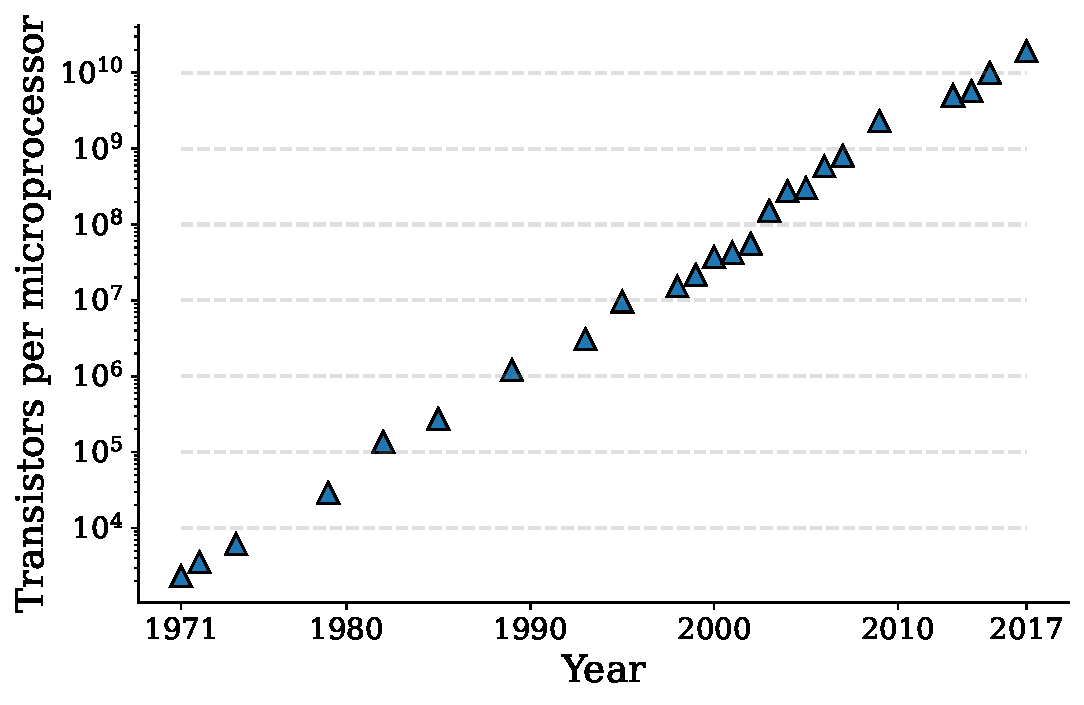
\includegraphics[width=0.8\textwidth]{lesson1/1-4_transistors.pdf}
    \caption[Moore's law.]{Number of transistors on a microprocessor has been doubling nearly every two years.}
    \label{fig:1-4_transistors}
\end{figure}

What are the two main ingredients that set quantum communication apart from its classical counterpart?
The first one is the \textit{\textbf{superposition principle}}.
This principle is not really anything new, as it is observed in the classical world as well.
We are all familiar with superposition of waves.
What is meant by superposition principle in quantum communication is the ability of quantum bits to be in a superposition of their usual classical states.
The possibility of a quantum bit to be both on and off at the same time is mind-bending but is at the heart of quantum communication.

Expanding the principle of superposition to multiple particles, we arrive at the concept of \textit{\textbf{entanglement}}.
Entanglement has no classical counterpart whatsoever.
It correlates distant quantum objects across large distances of space much more strongly than is possible using classical laws of nature.
The beauty of entanglement is that it allows for radically new ways to communicate and is used as a resource in quantum communication.
Distribution of entanglement is therefore one of the main jobs of quantum networks.

Is quantum communication difficult?
Quantum communication protocols are currently very difficult to implement.
Quantum systems are very delicate as they decohere extremely rapidly leading to loss of their quantum properties.
They go from being true and false at the same time, to being only true or only false.
Basically, they just become classical bits.

Quantum systems are difficult to build at the hardware level, but at the same time, it is also conceptually challenging to think about new ways of exploiting their quantum properties.
Designing new protocols for processing and communication in the quantum realm requires new tools.
It requires a completely new mental framework for how we approach problems, and how we solve problems.
This all seems very daunting but these challenges should be viewed as opportunities.
Quantum computation and quantum communication are vibrant and cross-disciplinary fields.
Engineers, physicists, mathematicians, and computer scientists are all working together on cracking difficult questions whose solutions will lead to incredible new quantum technologies.

\section{Security in the quantum age}

Quantum technologies carry the potential to impact a number of important areas.
Quantum simulation and computation are thought to bring about new methods in developing materials with novel and useful properties, as well as novel drugs.
Quantum metrology allows for measurements with unprecedented resolution and sensitivity.
Quantum machine learning aims to exploit the properties of quantum mechanics to enhance artificial intelligence.
Lastly, you may have heard that quantum computers will be able to crack some encryption schemes deployed currently.
This sounds like a doomsday scenario.
Since these lecture notes focus on quantum communication, we will briefly discuss what this claim means and show how quantum technologies can also enhance security.

\begin{figure}[t]
    \centering
    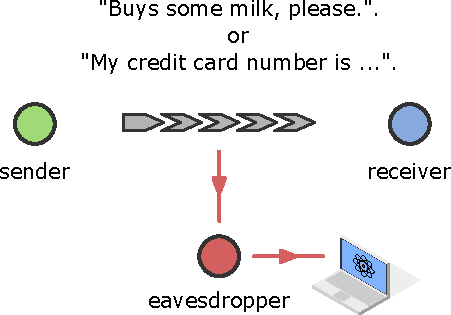
\includegraphics[width=0.5\textwidth]{lesson1/1-5_security.pdf}
    \caption[Security in the quantum age.]{An eavesdropper is trying to intercept and decrypt the message sent from the sender to the receiver.}
    \label{fig:1-5_security}
\end{figure}

Let's consider a sender wishing to send a message to a receiver as pictured in Fig.~\ref{fig:1-5_security}.
The message might be something mundane such as ``Buy some milk, please'' or might be something sensitive such as ``My credit card number is ...''.
Either way, messages sent over public channels are encrypted to preserve the privacy of the conversation between the sender and the receiver.
Let's consider a third party, an eavesdropper, who is trying to listen in on the conversation by intercepting the message.
Current classical encryption techniques offer \textit{\textbf{computational security}}, meaning that cracking them is not impossible, merely very difficult and would require enormous classical resources to do so.
Quantum algorithms exist that break this encryption.
An eavesdropper with access to a quantum computer could in principle intercept the encrypted message, use their quantum computer to break the code and listen in on the conversation with impunity.

To overcome this problem, the communicating parties need to resort to using \textit{\textbf{quantum key distribution}} (QKD).
With the help of the superposition principle or entanglement, the sender and the receiver can discover the eavesdropper's attempts to intercept and tamper with their messages.
They can then simply not transmit their sensitive message.
This method of encryption offers \textit{\textbf{information-theoretic security}}.
Such security does not rely on the computational difficulty of certain mathematical problems and therefore is stronger than the computational security used currently.
For this reason, QKD is one of the primary applications of quantum networks.
We will explore the basics of QKD later in this book.

\section{Module Overview}
\label{sec:mod-over}

Before concluding the first chapter, let's have a brief look at the structure of this module.
The next three chapters deal with the basics of quantum mechanics relevant to quantum communication.
We will learn about quantum bits and how they are different from classical bits, consider how noise affects the state of quantum states and how we can describe this effect mathematically.
Finally, we will look at systems of multiple quantum bits.

Chapters 5-7 deal with the basics of optics.
Light is an excellent information carrier and we will learn how lasers produce light.
We will discuss interference, one of the fundamental phenomena in both classical as well as quantum physics.
We will conclude this block of chapters by learning about waveguides and how light is guided in a network.

Chapters 8-10 look at fundamental quantum communication protocols.
We will learn how teleportation can be used to transmit information without sending the physical system encoding this information as well as how quantum key distribution works.

In chapters 11-13, we will look at the basics of quantum repeaters, a quantum technology that makes long-distance quantum communication possible.
The last two chapters look at quantum repeater systems.

There are some basic prerequisites for this module such as linear algebra (meaning vector and matrix multiplication; eigenvectors and eigenvalues; also, we will use the tensor product which will be introduced in this book), discrete probability, and complex numbers (e.g., $i = \sqrt{-1}$ and Euler's equation, $e^{i\pi} + 1 = 0$). It's very helpful if you have some introduction to quantum computing; programming and classical computing; and computer networks.
Other than that there are no physics requirements.

If you don't have some of this background yet, there are a lot of online materials, particularly our MOOC (massively open online course), "Understanding Quantum Computers", which is targeted at learners at the high school level and requires very minimal math.
It is available in English, Japanese, Thai and Indonesian.
If you would like to learn a little bit more about some basic linear algebra you can have a look at the playlist on Professor Van Meter's YouTube channel. There are many other courses available. Other modules from the Quantum Academy of Science and Technology (supported by the Q-Leap Education office in Japan) cover some of this background material as well, and may be available to you.


% \begin{figure}[H]
%     \centering
%     \includegraphics[width=0.9\textwidth]{lesson1/communication.eps}
%     \label{fig:1-1}
%     \caption{Evolution of communication.}
% \end{figure}

% insert photo here
% \begin{figure}[H]
%     \centering
%     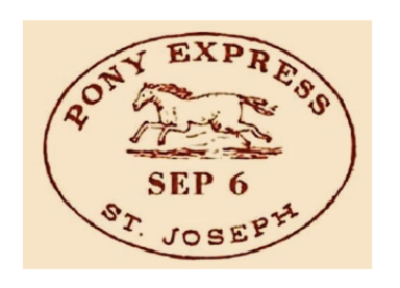
\includegraphics[width=0.6\textwidth]{lesson1/ponyexpress.eps}
%     \label{fig:1-2}
%     %\justification=<centering>
%     \caption{Pony Express.}
% \end{figure}

% insert photo here
% \begin{figure}[H]
%     \centering
%     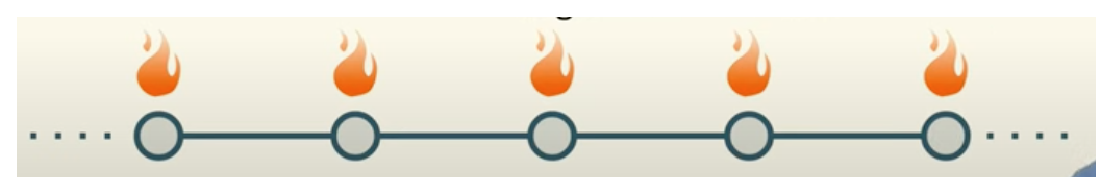
\includegraphics[width=0.9\textwidth]{lesson1/万里の長城.eps}
%     \label{fig:1-3}
%     \caption{The Great Wall of China.}
% \end{figure}

% Insert photo here
% \begin{figure}[H]
%     \centering
%     \includegraphics[width=0.9\textwidth]{lesson1/napoleon.eps}
%     \label{fig:1-4}
%     \caption{Napoleon's semaphore.}
% \end{figure}

% insert photo here. TODO: How to make these side-by-side?
% \begin{figure}[H]
%     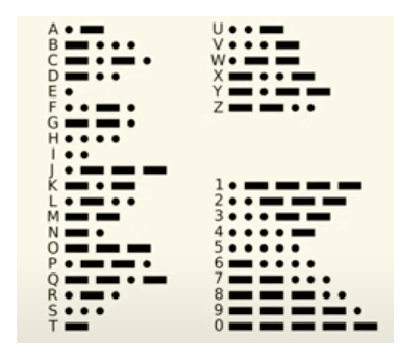
\includegraphics[width=0.3\textwidth]{lesson1/morse.eps}
%     \label{fig:1-5}
%     \caption{Morse signal.}
% \end{figure}
% \begin{figure}[H]
%     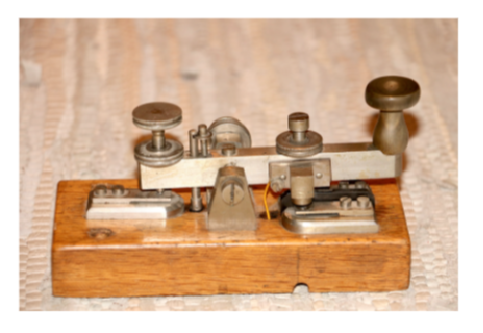
\includegraphics[width=0.3\textwidth]{lesson1/morsekey.eps}
%     \label{fig:1-6}
%     \caption{Morse key.}
% \end{figure}
% \iffalse
% \begin{figure}
%     \centering
%     \begin{minipage}{0.45\textwidth}
%         \centering
%         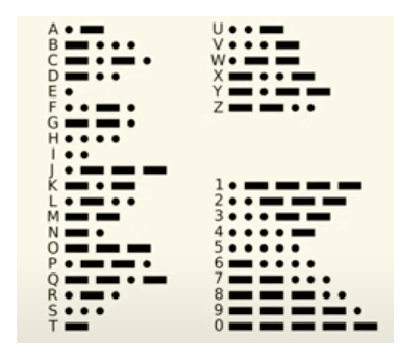
\includegraphics[width=0.9\textwidth]{lesson1/morse.eps} % first figure itself
%         \caption{first figure}
%     \end{minipage}\hfill
%     \begin{minipage}{0.45\textwidth}
%         \centering
%         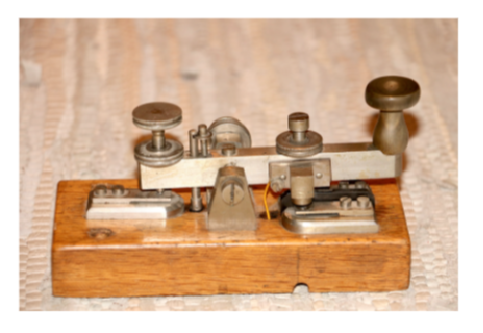
\includegraphics[width=0.9\textwidth]{lesson1/morsekey.eps} % second figure itself
%         \caption{second figure}
%     \end{minipage}
% \end{figure}
% \fi

% Insert point-to-point pic here
% \begin{figure}[H]
%     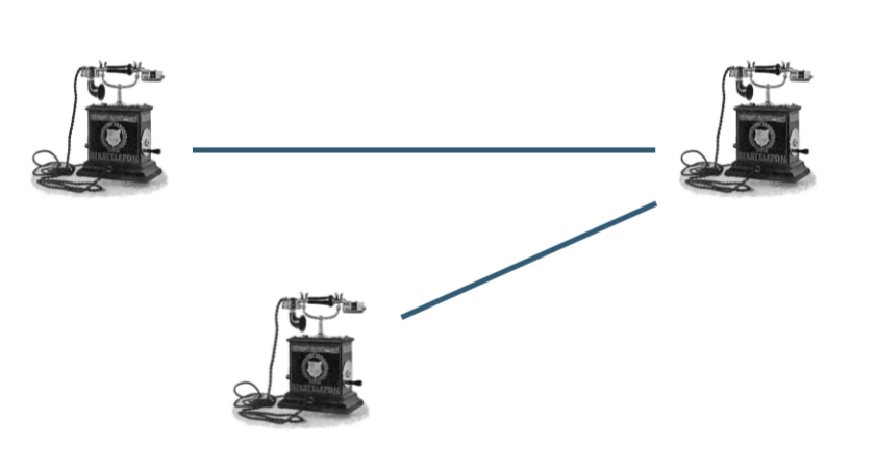
\includegraphics[width=0.8\textwidth]{lesson1/pointpoint.eps}
%     \label{fig:1-7}
%     \caption{Point-to-point.}
% \end{figure}

% Insert switchboard pic here.
% \begin{figure}[H]
%     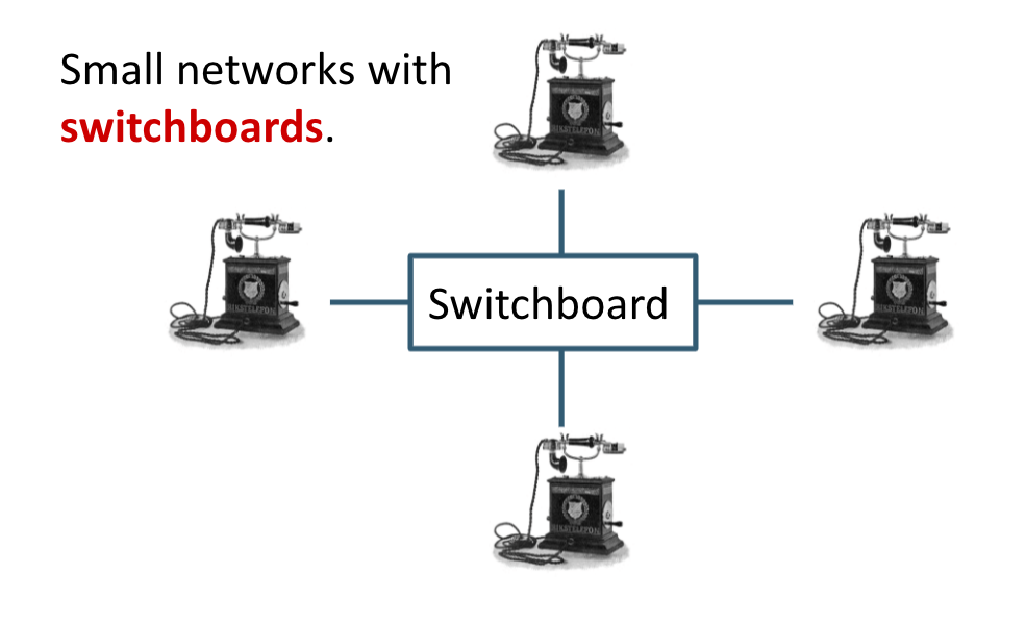
\includegraphics[width=0.8\textwidth]{lesson1/switchboard.eps}
%     \label{fig:1-8}
%     \caption{Switchboard.}
% \end{figure}
% insert internet pic here
% \begin{figure}[H]
%     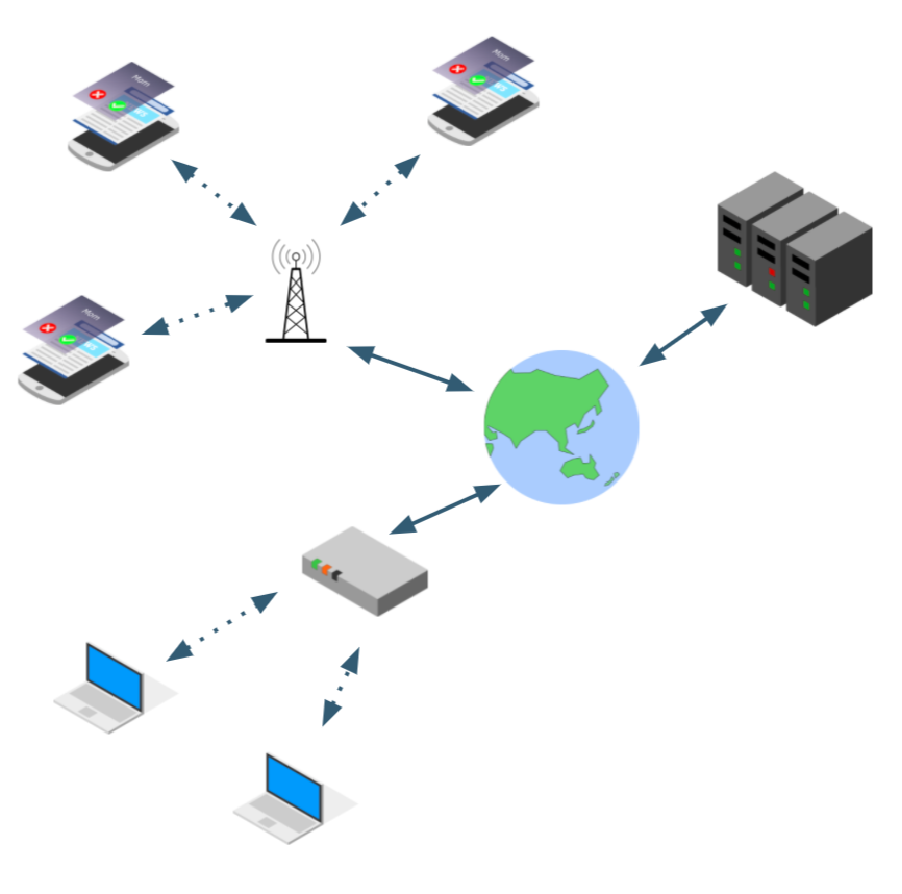
\includegraphics[width=0.8\textwidth]{lesson1/internet.eps}
%     \label{fig:1-9}
%     \caption{The Internet.}
% \end{figure}
% insert picture here
% \begin{figure}[H]
%     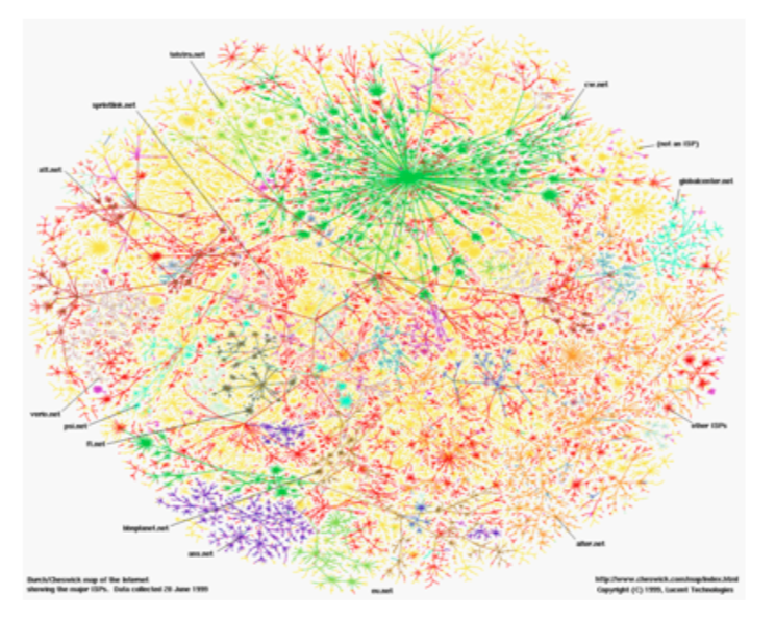
\includegraphics[width=0.8\textwidth]{lesson1/internetmap.eps}
%     \label{fig:1-10}
%     \caption{Network of networks.}
% \end{figure}

% \begin{figure}[H]
%     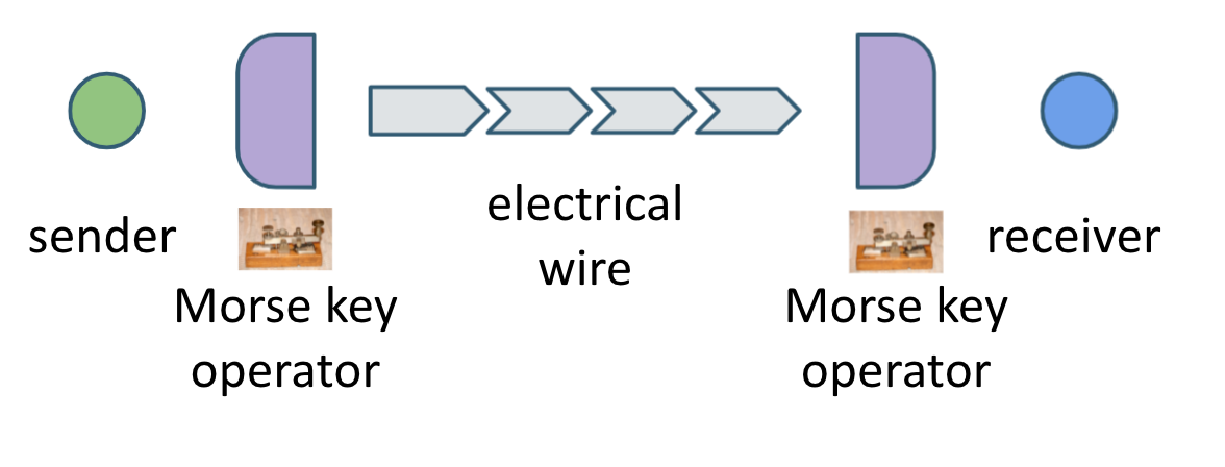
\includegraphics[width=0.8\textwidth]{lesson1/sender_receiver.eps}
%     \label{fig:1-11}
%     \caption{Sender and receiver.}
% \end{figure}


% insert continuous signal picture.
% \begin{figure}[H]
%     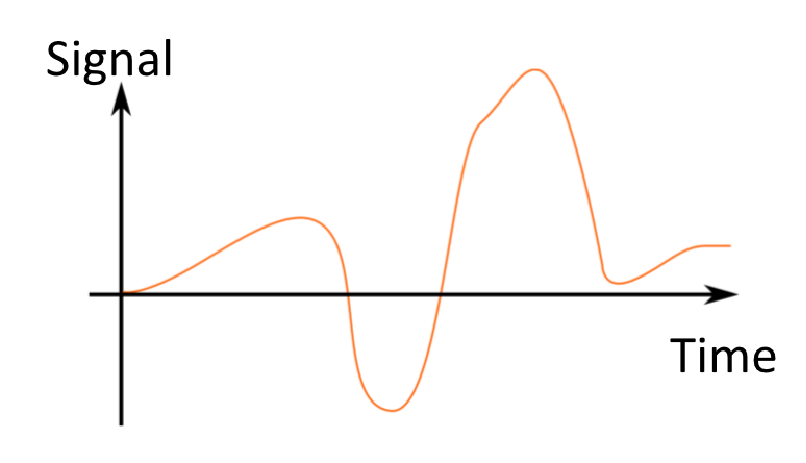
\includegraphics[width=0.8\textwidth]{lesson1/continuoussignal.eps}
%     \label{fig:1-12}
%     \caption{Analog communication}
% \end{figure}

% insert continuous signal w/ disruptive noise included here. 
% \begin{figure}[H]
%     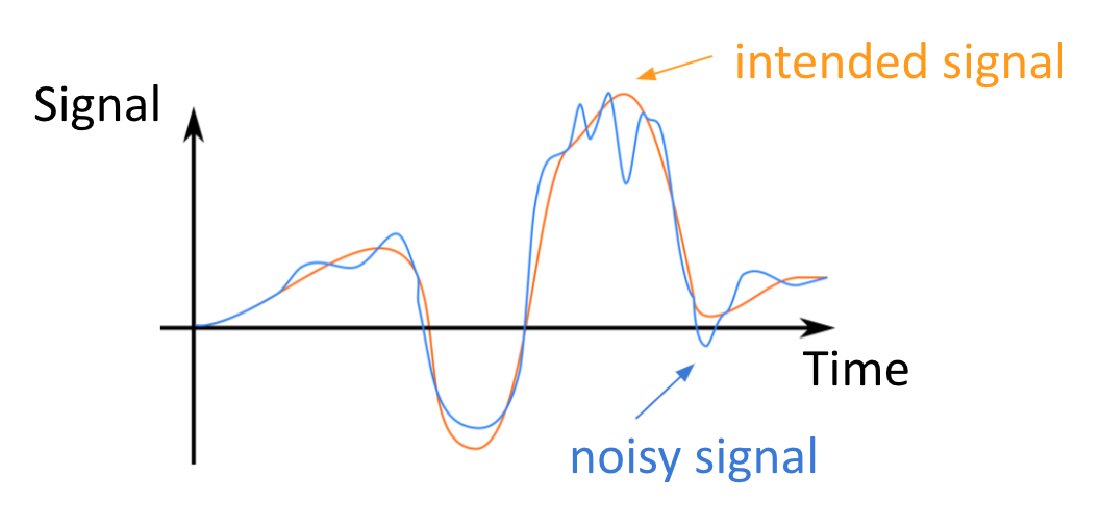
\includegraphics[width=0.8\textwidth]{lesson1/continuous_signal_noise.eps}
%     \label{fig:1-13}
%     \caption{Analog signal and noise.}
% \end{figure}

% Insert discrete digital signal pic  w/ t_0, t_1, t_2 here
% \begin{figure}[H]
%     \centering
%     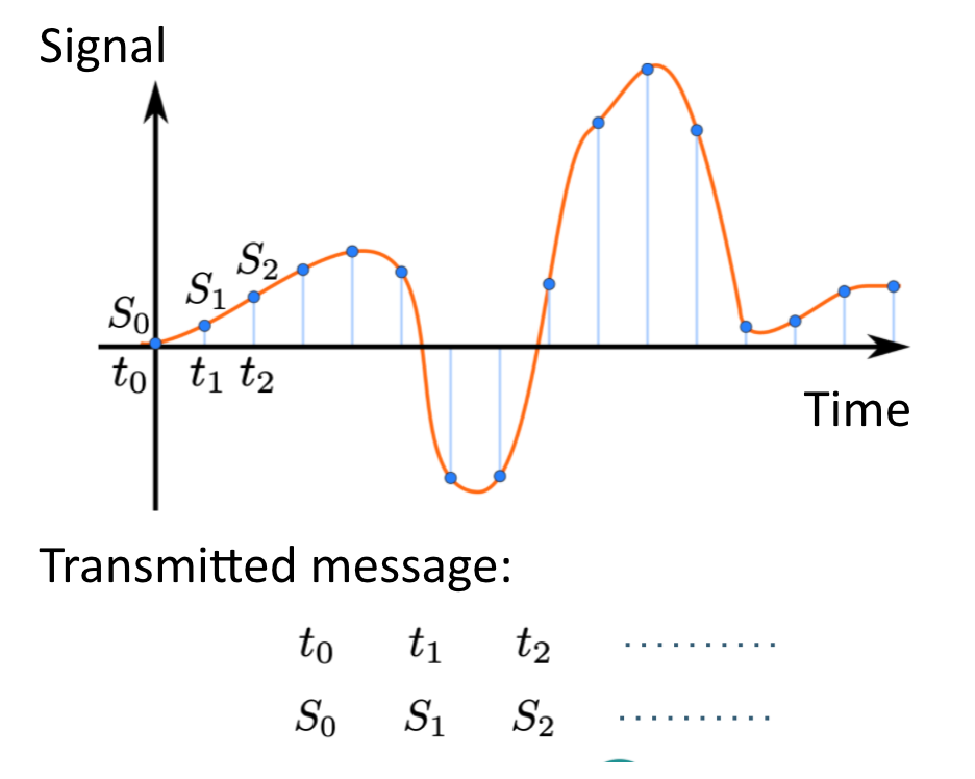
\includegraphics[width=0.8\textwidth]{lesson1/discre_signal.eps}
%     \label{fig:1-14}
%     \begin{center}
%         \caption{Discrete signals.}
%     \end{center}
% \end{figure}

% insert war is over
% \begin{figure}[H]
%     \centering
%     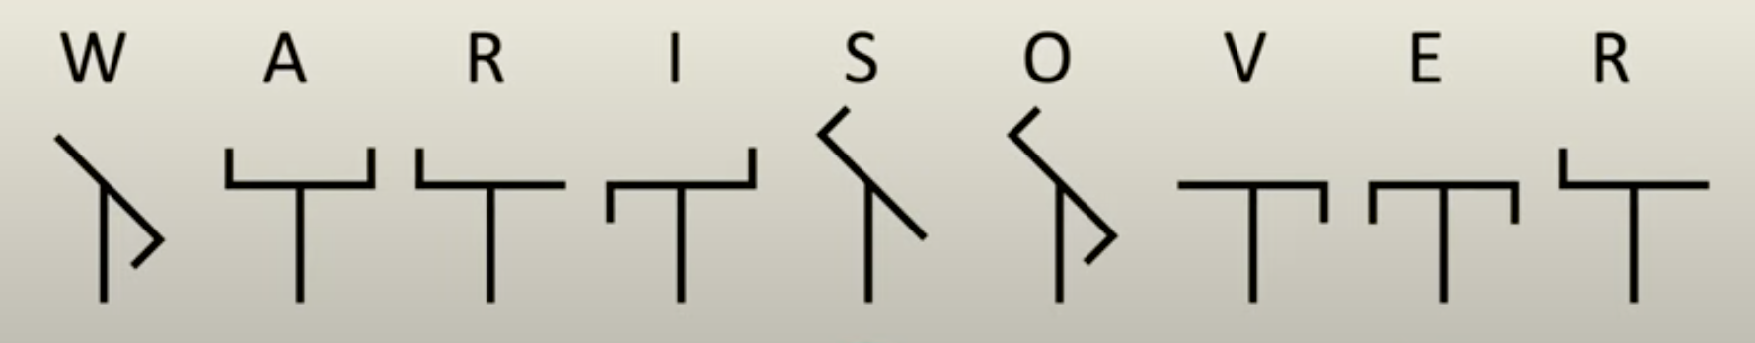
\includegraphics[width=0.5\textwidth]{lesson1/warisover.pdf}
%     \label{fig:1-15}
%     \begin{center}
%         \caption{Letters spelling "War is over".}
%     \end{center}
% \end{figure}

% Insert A -> R, W -> 10 
% \begin{figure}[H]
%     \centering
%     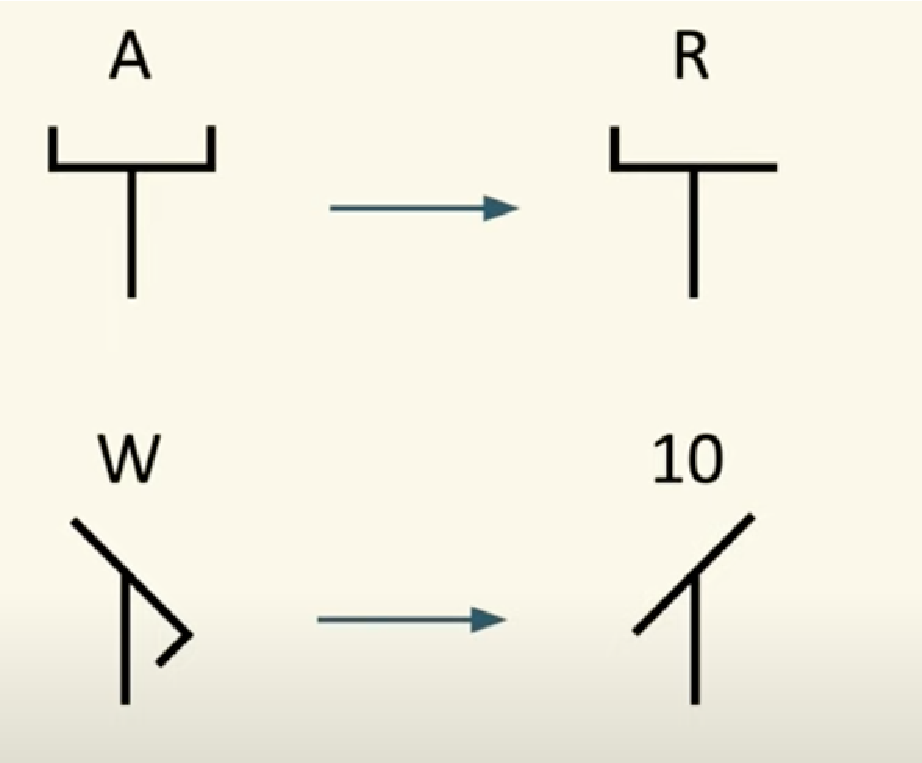
\includegraphics[width=0.8\textwidth]{lesson1/a_to_r.pdf}
%     \label{fig:1-16}
%     \begin{center}
%         \caption{Letters.}
%     \end{center}
% \end{figure}

% Insert U encoding
% \begin{figure}[H]
%     \centering
%     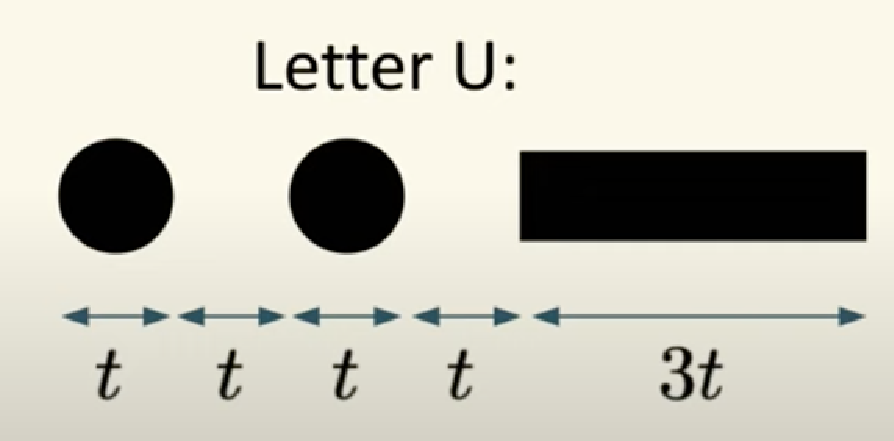
\includegraphics[width=0.8\textwidth]{lesson1/letter_u.pdf}
%     \label{fig:1-17}
%     \begin{center}
%         \caption{Morse code letter U.}
%     \end{center}
% \end{figure}

% insert morse graph
% \begin{figure}[H]
%     \centering
%     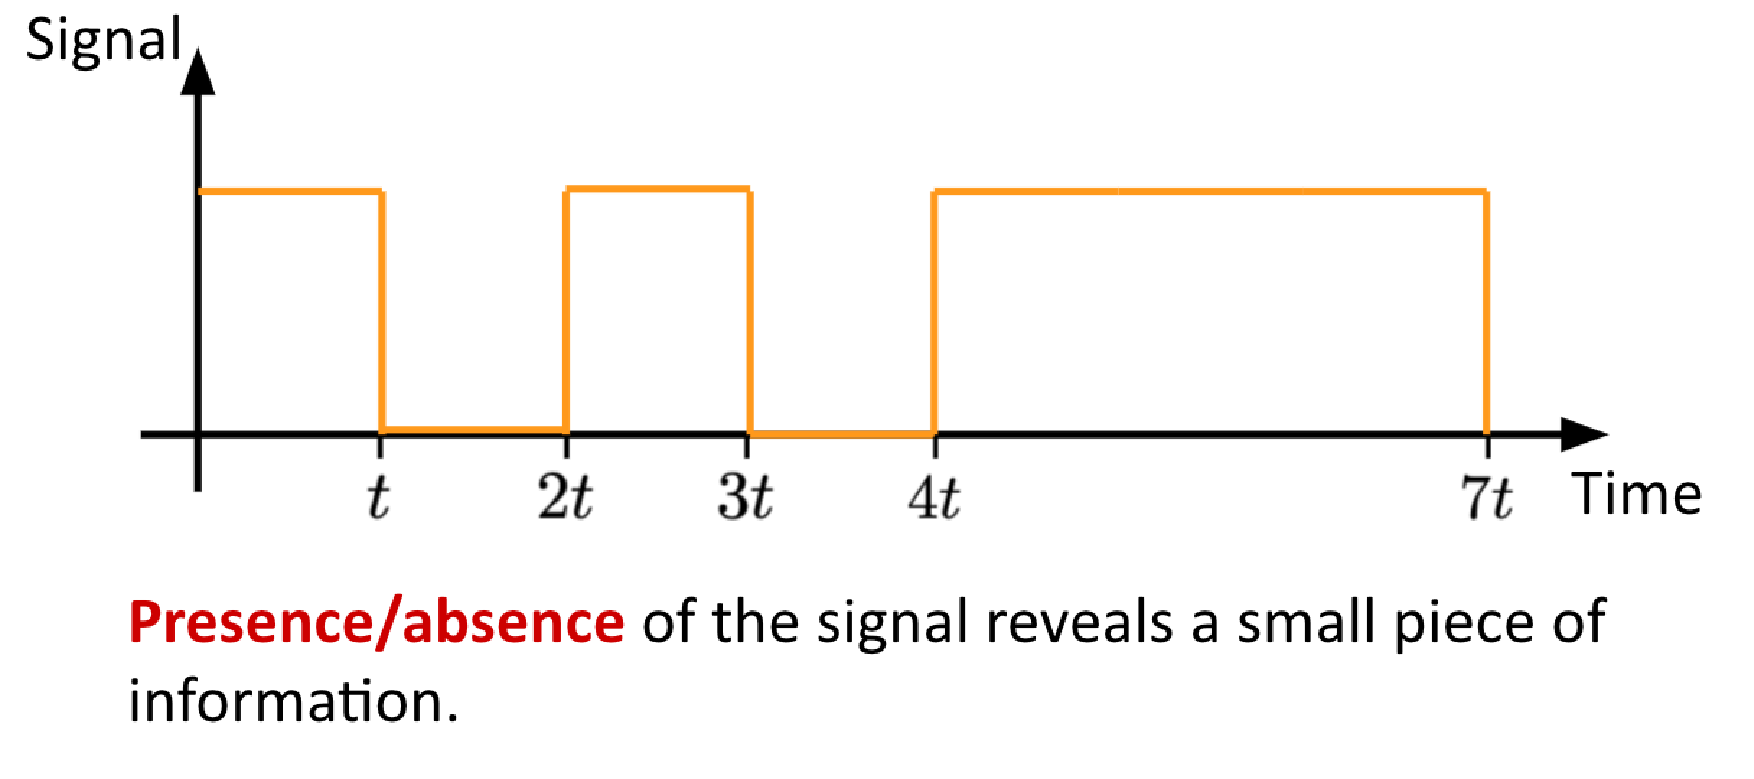
\includegraphics[width=0.8\textwidth]{lesson1/presence_abscence.pdf}
%     \label{fig:1-18}
%     \begin{center}
%         \caption{Morse code.}
%     \end{center}
% \end{figure}

% \begin{figure}[H]
%     \centering
%     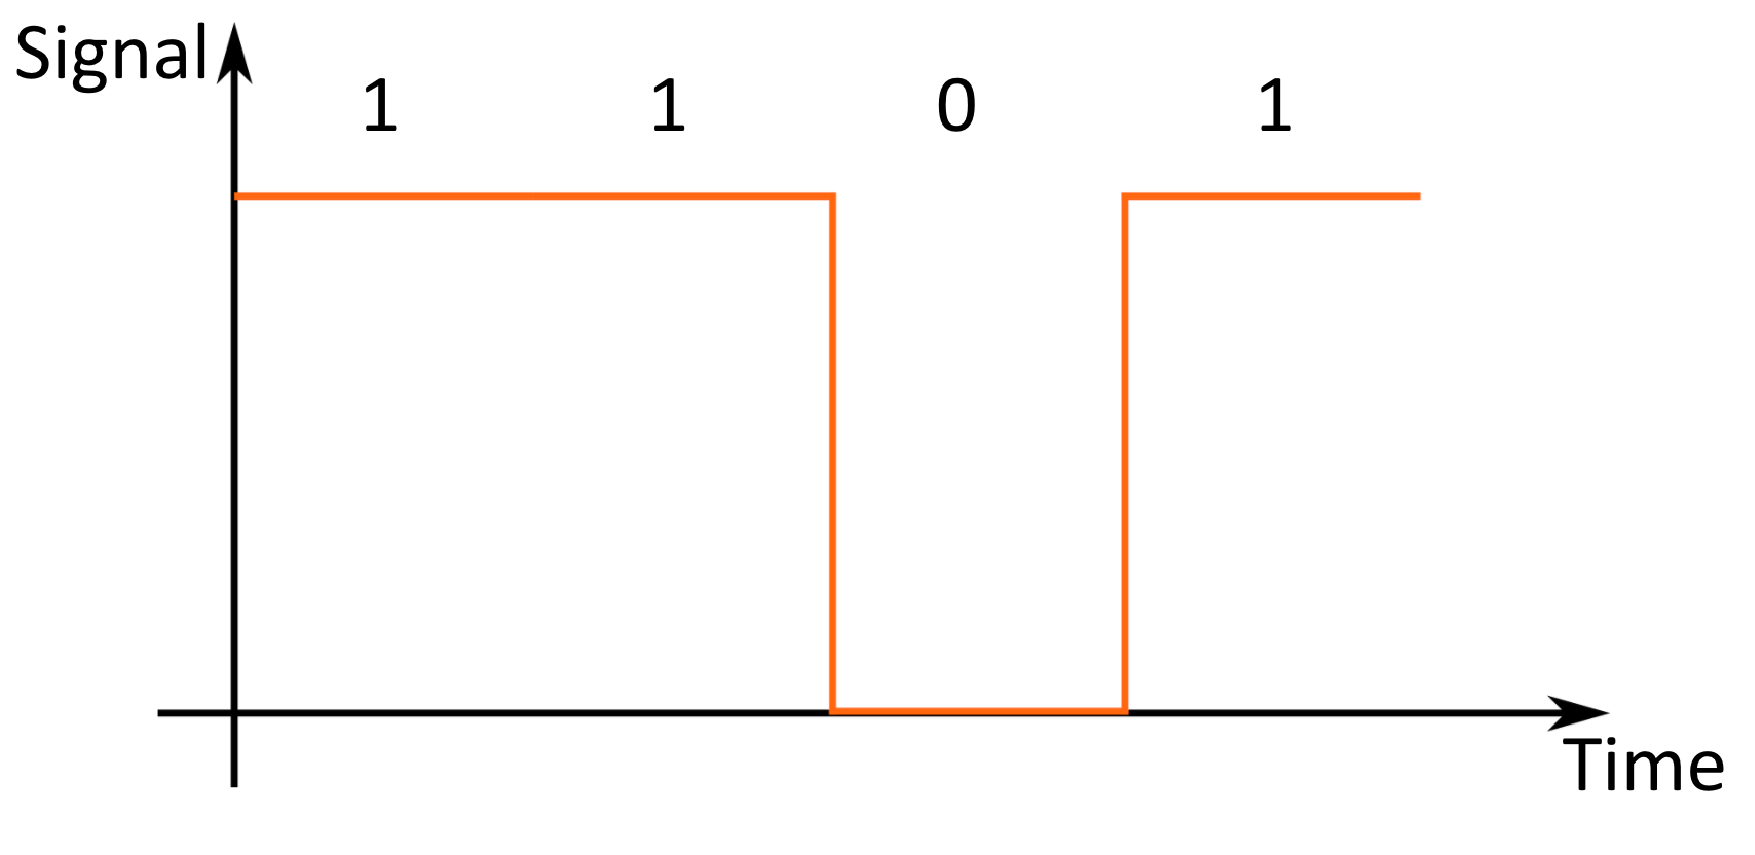
\includegraphics[width=0.8\textwidth]{lesson1/presence_abscence_bit.pdf}
%     \label{fig:1-19}
%     \begin{center}
%         \caption{Bits.}
%     \end{center}
% \end{figure}
% insert graph w/ noise
% \begin{figure}[H]
%     \centering
%     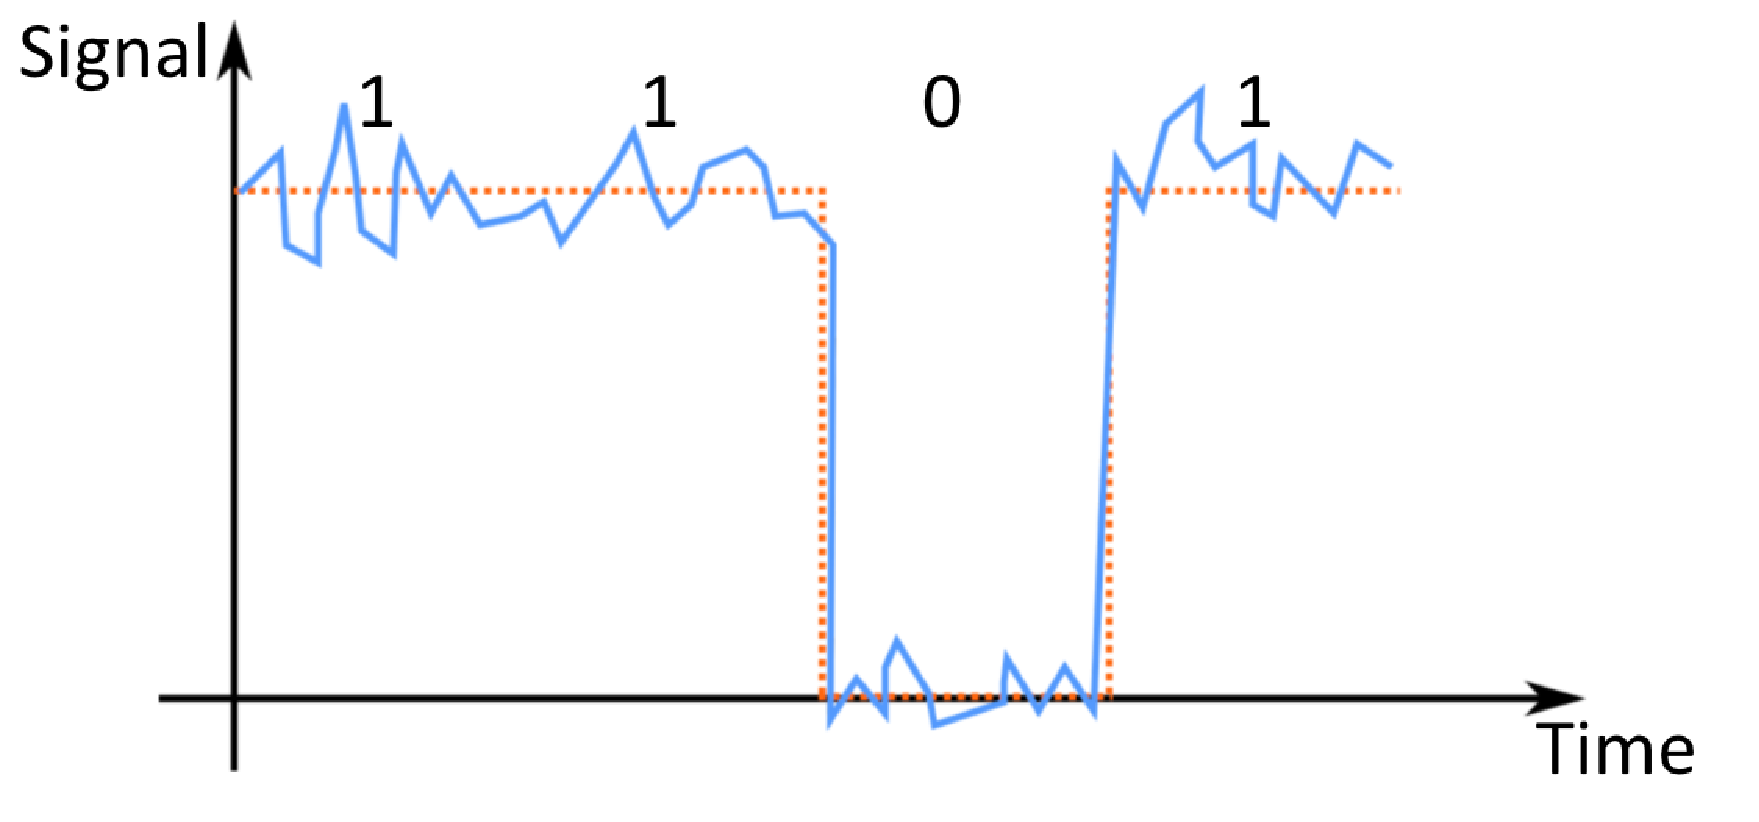
\includegraphics[width=0.8\textwidth]{lesson1/presence_abscence_noise.pdf}
%     \label{fig:1-20}
%     \begin{center}
%         \caption{Presence or absence as a bit.}
%     \end{center}
% \end{figure}

% insert bit permutations slide
% \begin{figure}[H]
%     \centering
%     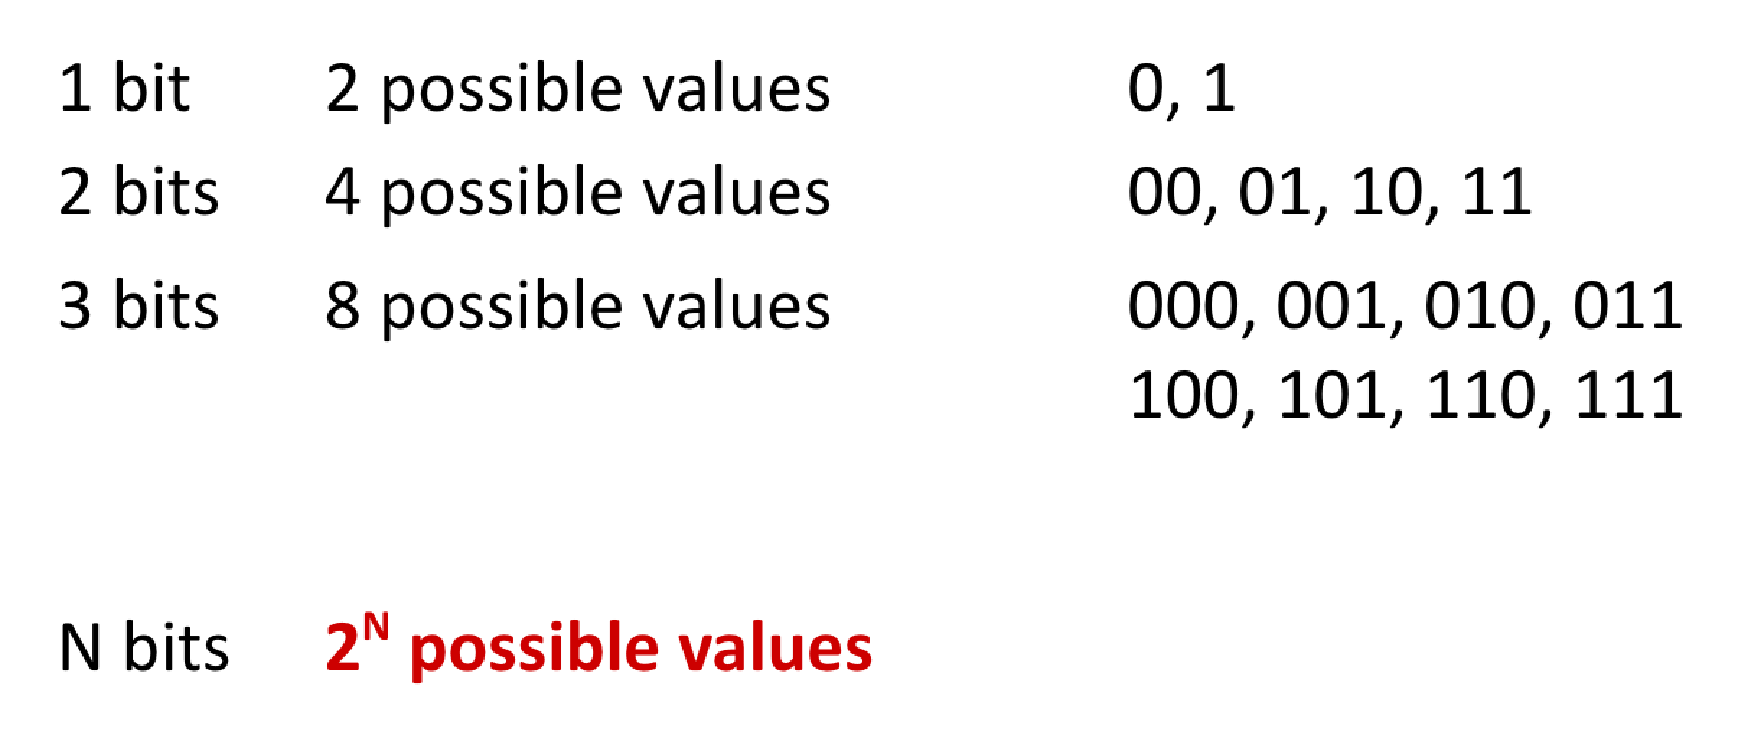
\includegraphics[width=0.8\textwidth]{lesson1/binary_notation.pdf}
%     \label{fig:1-21}
%     \begin{center}
%         \caption{Binary notation.}
%     \end{center}
% \end{figure}

% insert decimal notation
% \begin{figure}[H]
%     \centering
%     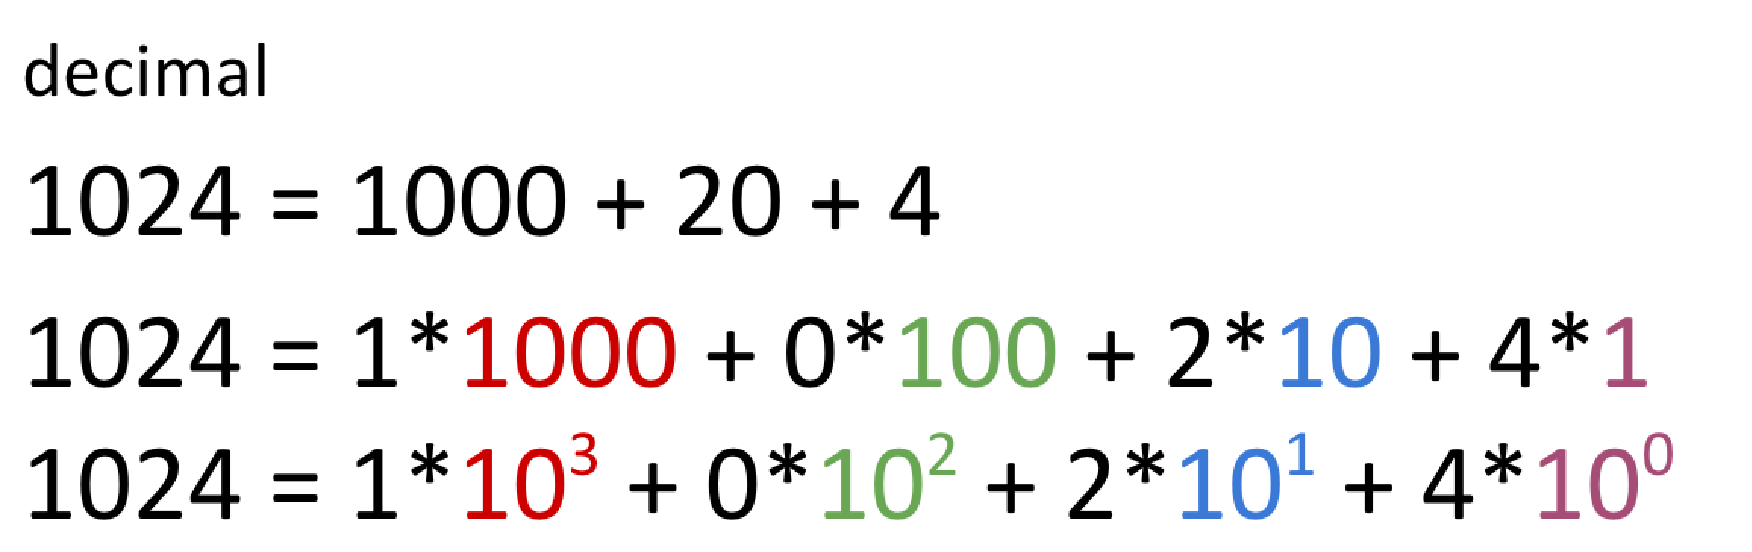
\includegraphics[width=0.8\textwidth]{lesson1/decimal_notation.pdf}
%     \label{fig:1-22}
%     \begin{center}
%         \caption{Decimal notation.}
%     \end{center}
% \end{figure}

% insert binary notation
% \begin{figure}[H]
%     \centering
%     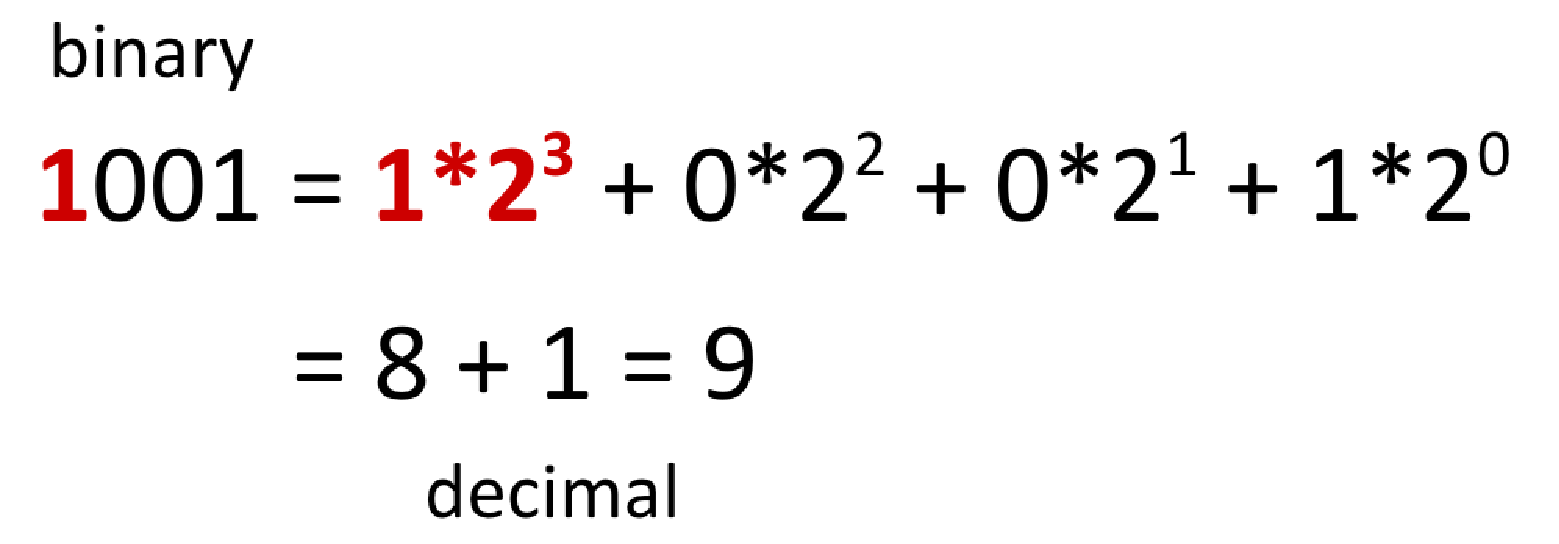
\includegraphics[width=0.8\textwidth]{lesson1/binary_ex.pdf}
%     \label{fig:1-23}
%     \begin{center}
%         \caption{Binary notation.}
%     \end{center}
% \end{figure}

% Insert classical VS quantum slide
% \begin{figure}[H]
%     \centering
%     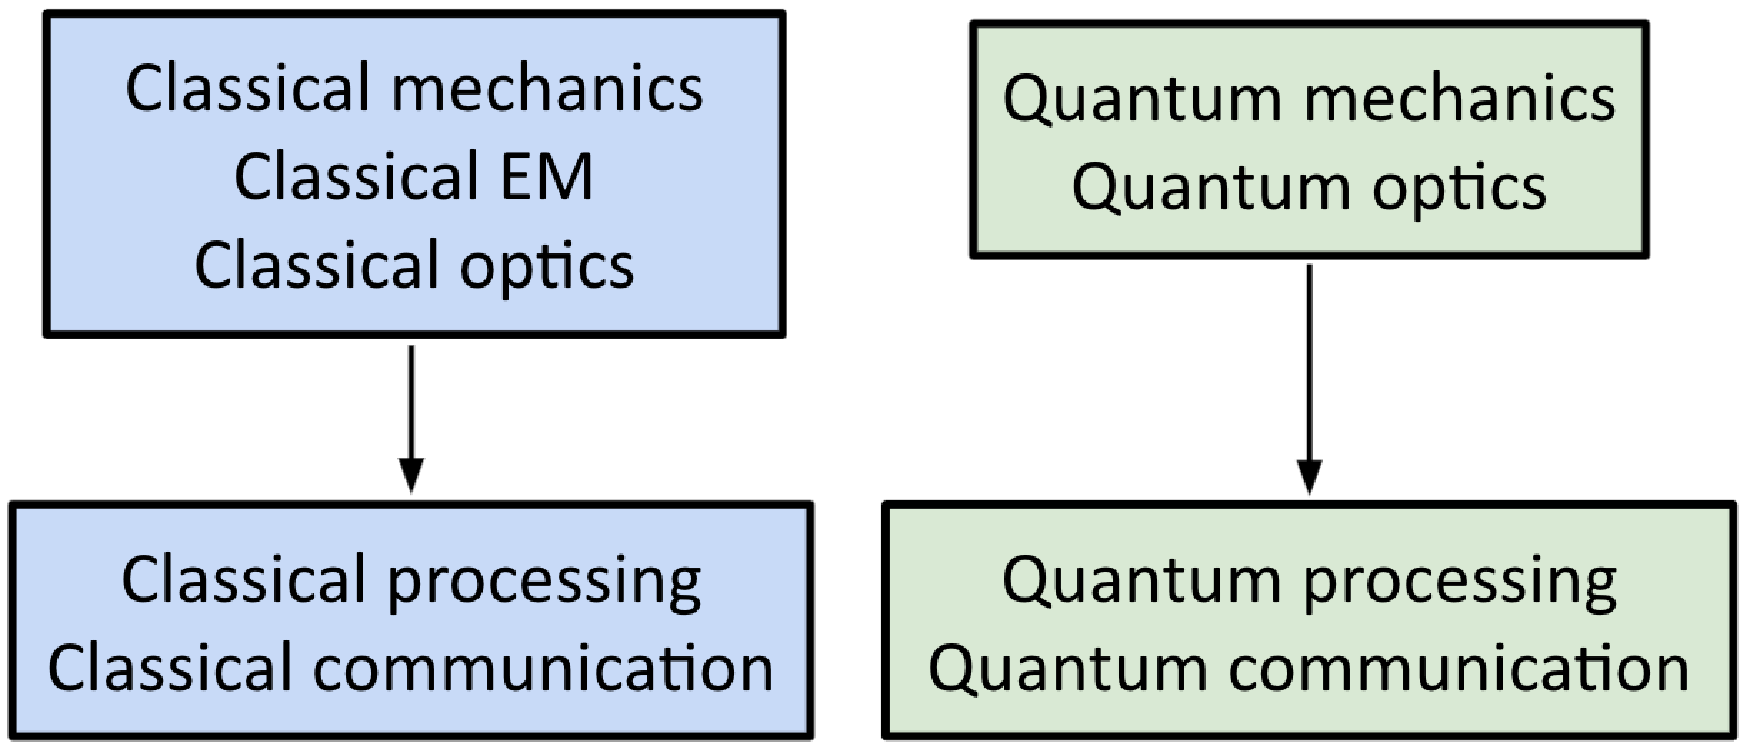
\includegraphics[width=0.8\textwidth]{lesson1/comparsion.pdf}
%     \label{fig:1-24}
%     \begin{center}
%         \caption{Classical and quantum.}
%     \end{center}
% \end{figure}

% Moore's law graph
% \begin{figure}[H]
%     \centering
%     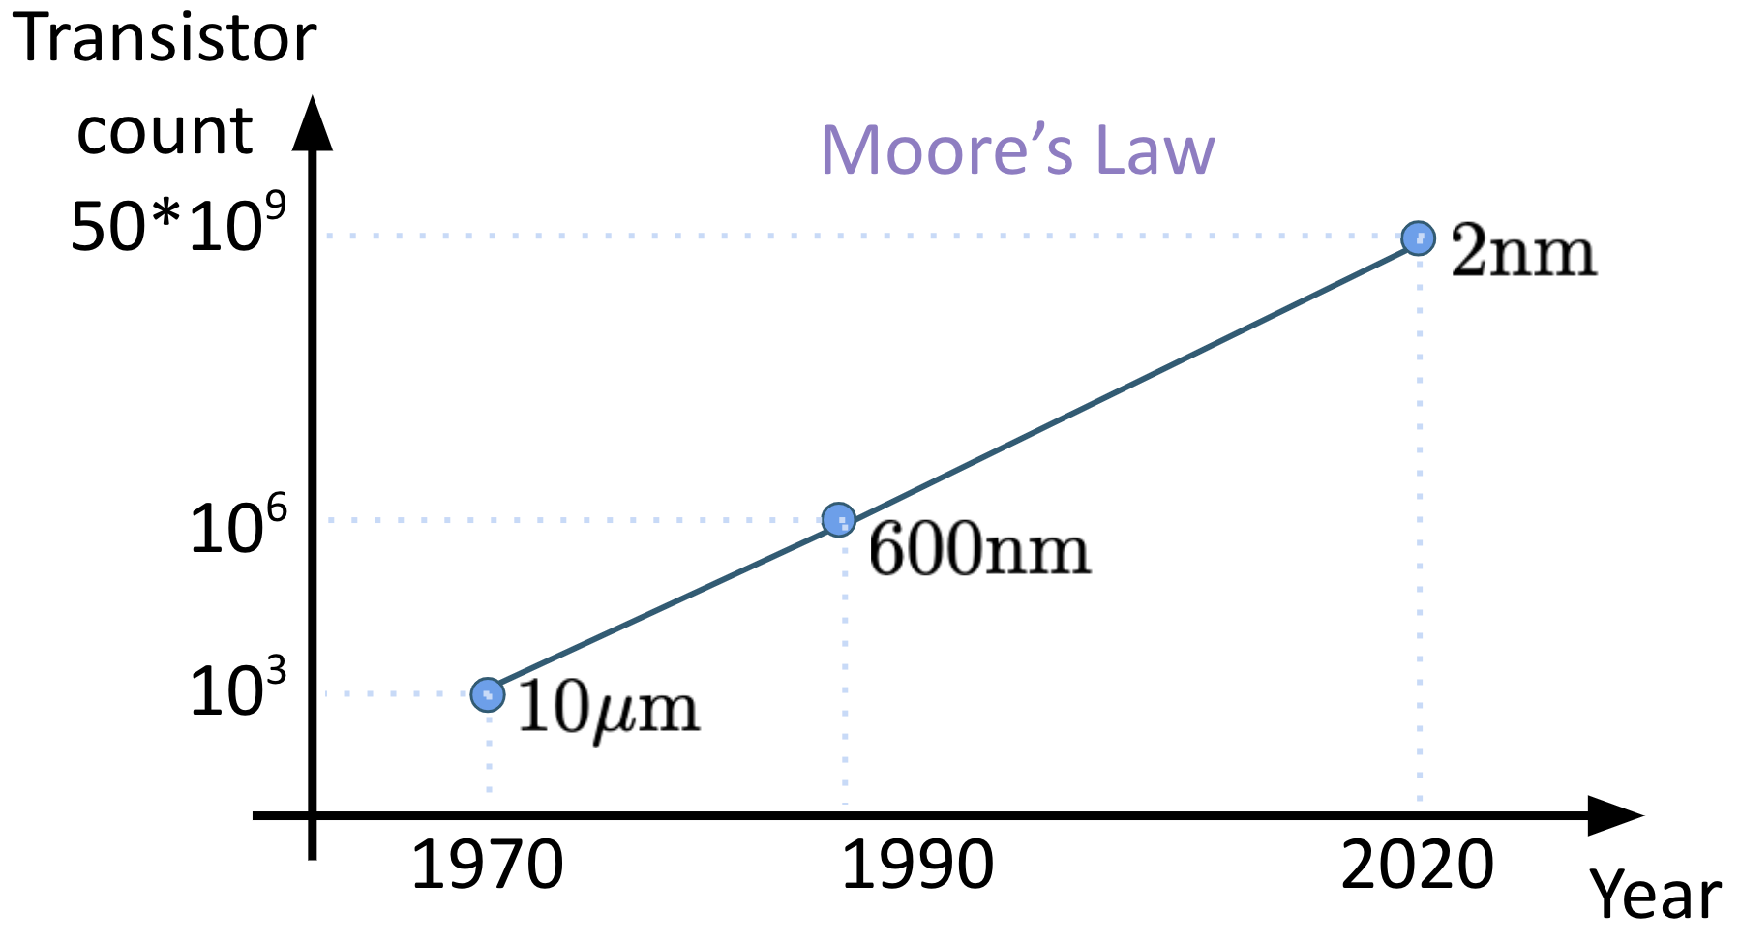
\includegraphics[width=0.8\textwidth]{lesson1/moore_law.pdf}
%     \label{fig:1-25}
%     \begin{center}
%         \caption{Moore's Law.}
%     \end{center}
% \end{figure}




% insert unencrytped msg pic (milk please)
% 

% insert credit card info 
% \begin{figure}[H]
%     \centering
%     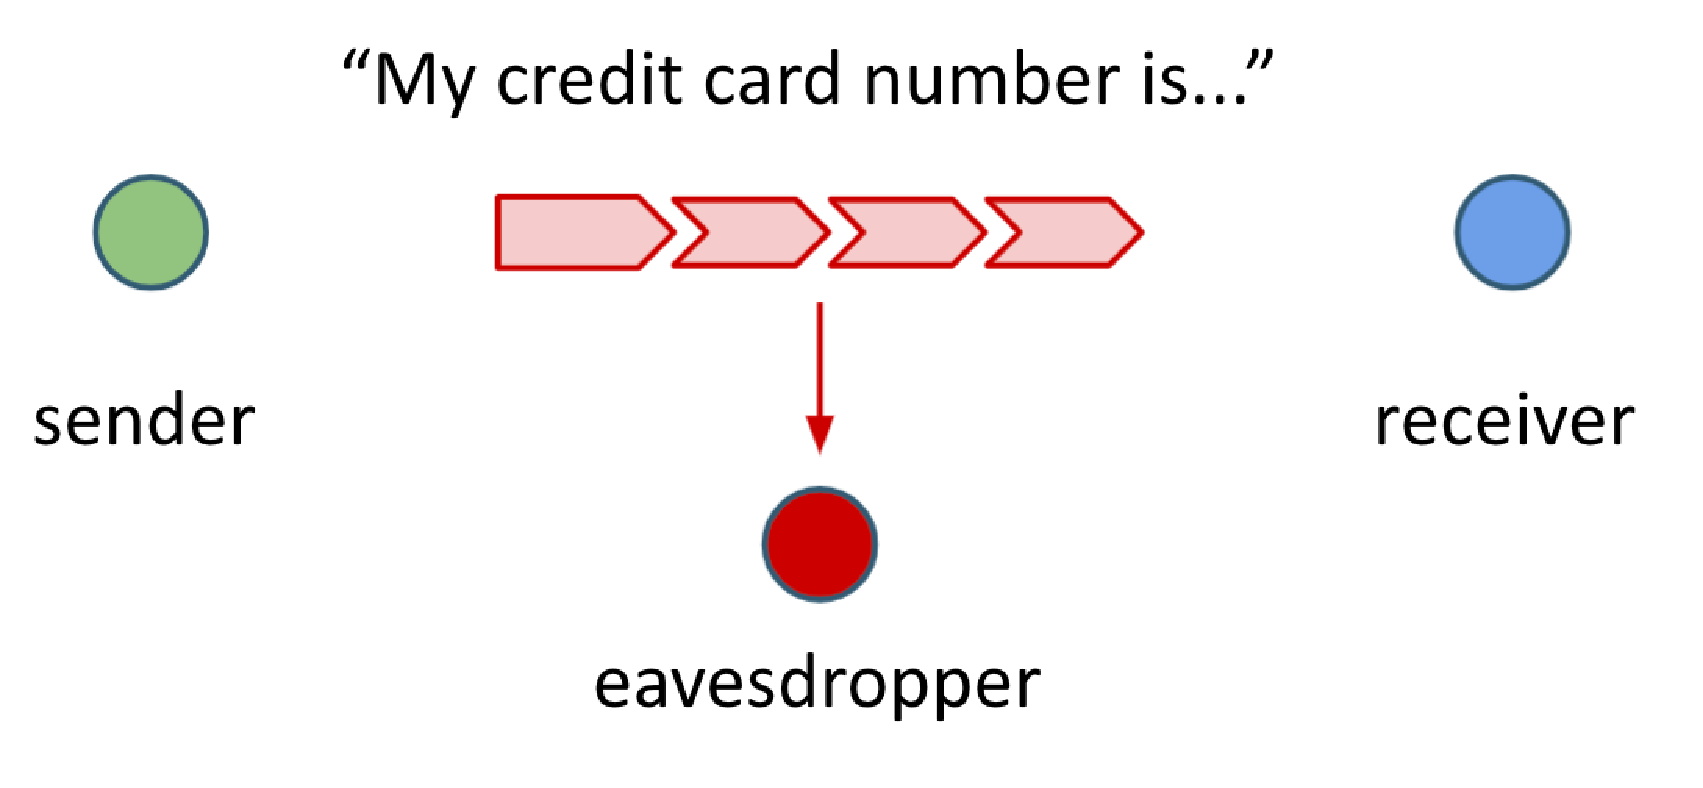
\includegraphics[width=0.8\textwidth]{lesson1/creditcardinfo.pdf}
%     \label{fig:1-26}
%     \begin{center}
%         \caption{Unencrypted communication: an eavesdropper overhearing your credit card information is much more likely to be a problem.}
%     \end{center}
% \end{figure}
% encrypted msg pic.
% \begin{figure}[H]
%     \centering
%     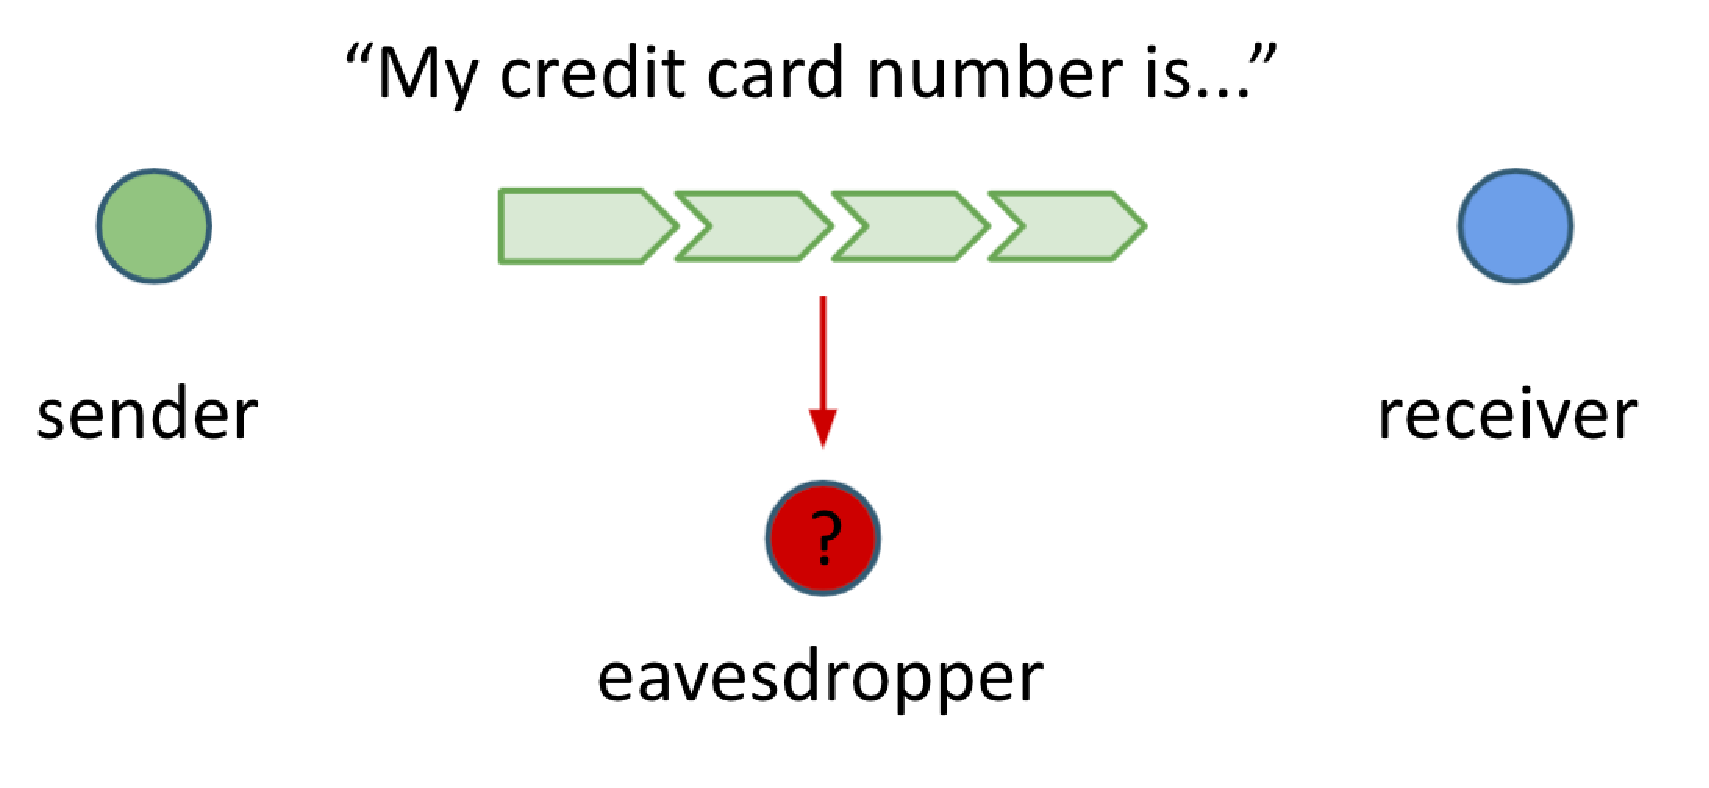
\includegraphics[width=0.8\textwidth]{lesson1/credit_card_info_eavesdropper.pdf}
%     \label{fig:1-28}
%     \begin{center}
%         \caption{Encrypted communication.}
%     \end{center}
% \end{figure}

% insecure channel pic.
% \begin{figure}[H]
%     \centering
%     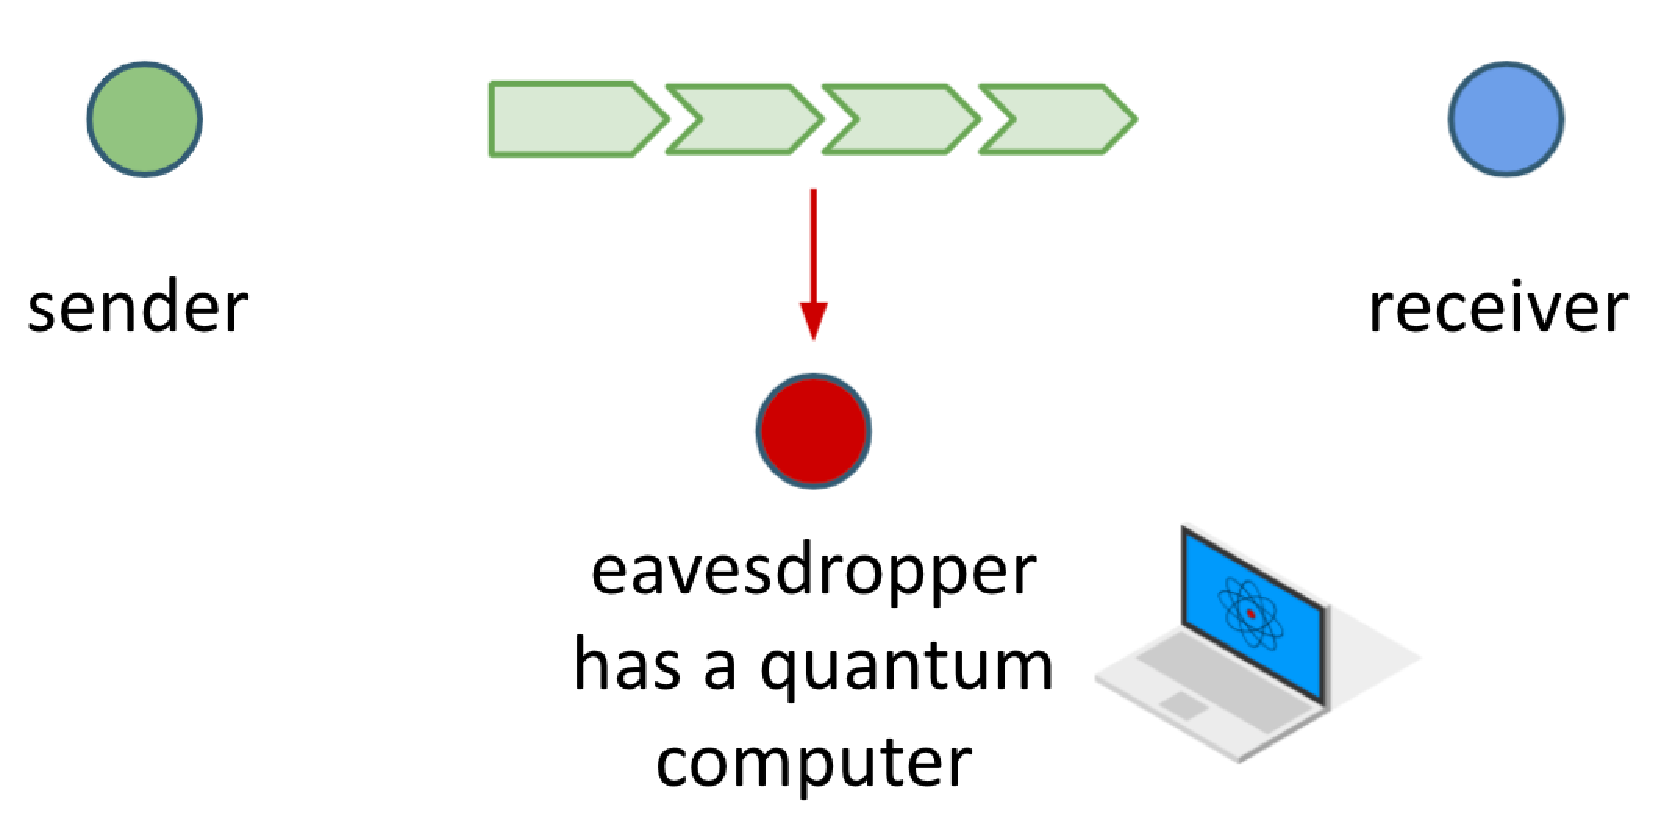
\includegraphics[width=0.8\textwidth]{lesson1/eavesdropper_Q_comp.pdf}
%     \label{fig:1-29}
%     \begin{center}
%         \caption{Eavesdropper with a quantum computer.}
%     \end{center}
% \end{figure}

% Quantum Channel "STOP" pic
% \begin{figure}[H]
%     \centering
%     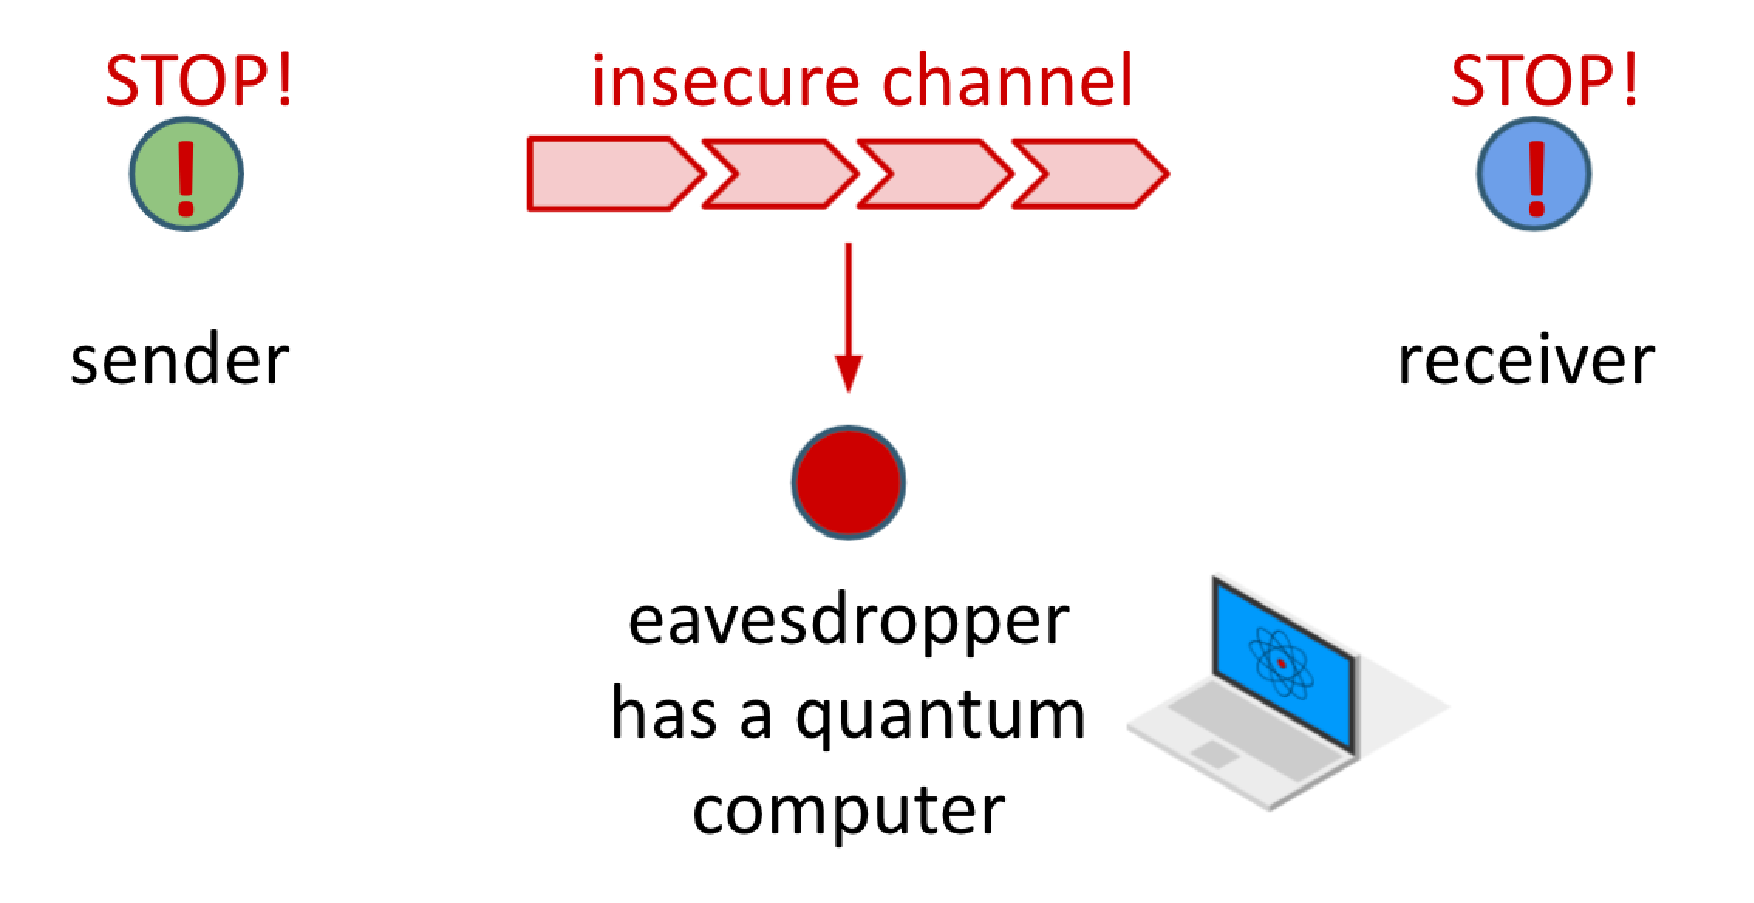
\includegraphics[width=0.8\textwidth]{lesson1/insecure_channel_stop.pdf}
%     \label{fig:1-30}
%     \begin{center}
%         \caption{Insecure quantum channel stops.}
%     \end{center}
% \end{figure}



% \section{(XXX Is a section break needed here?)}


% insert course overview pic
% \begin{figure}[H]
%     \centering
%     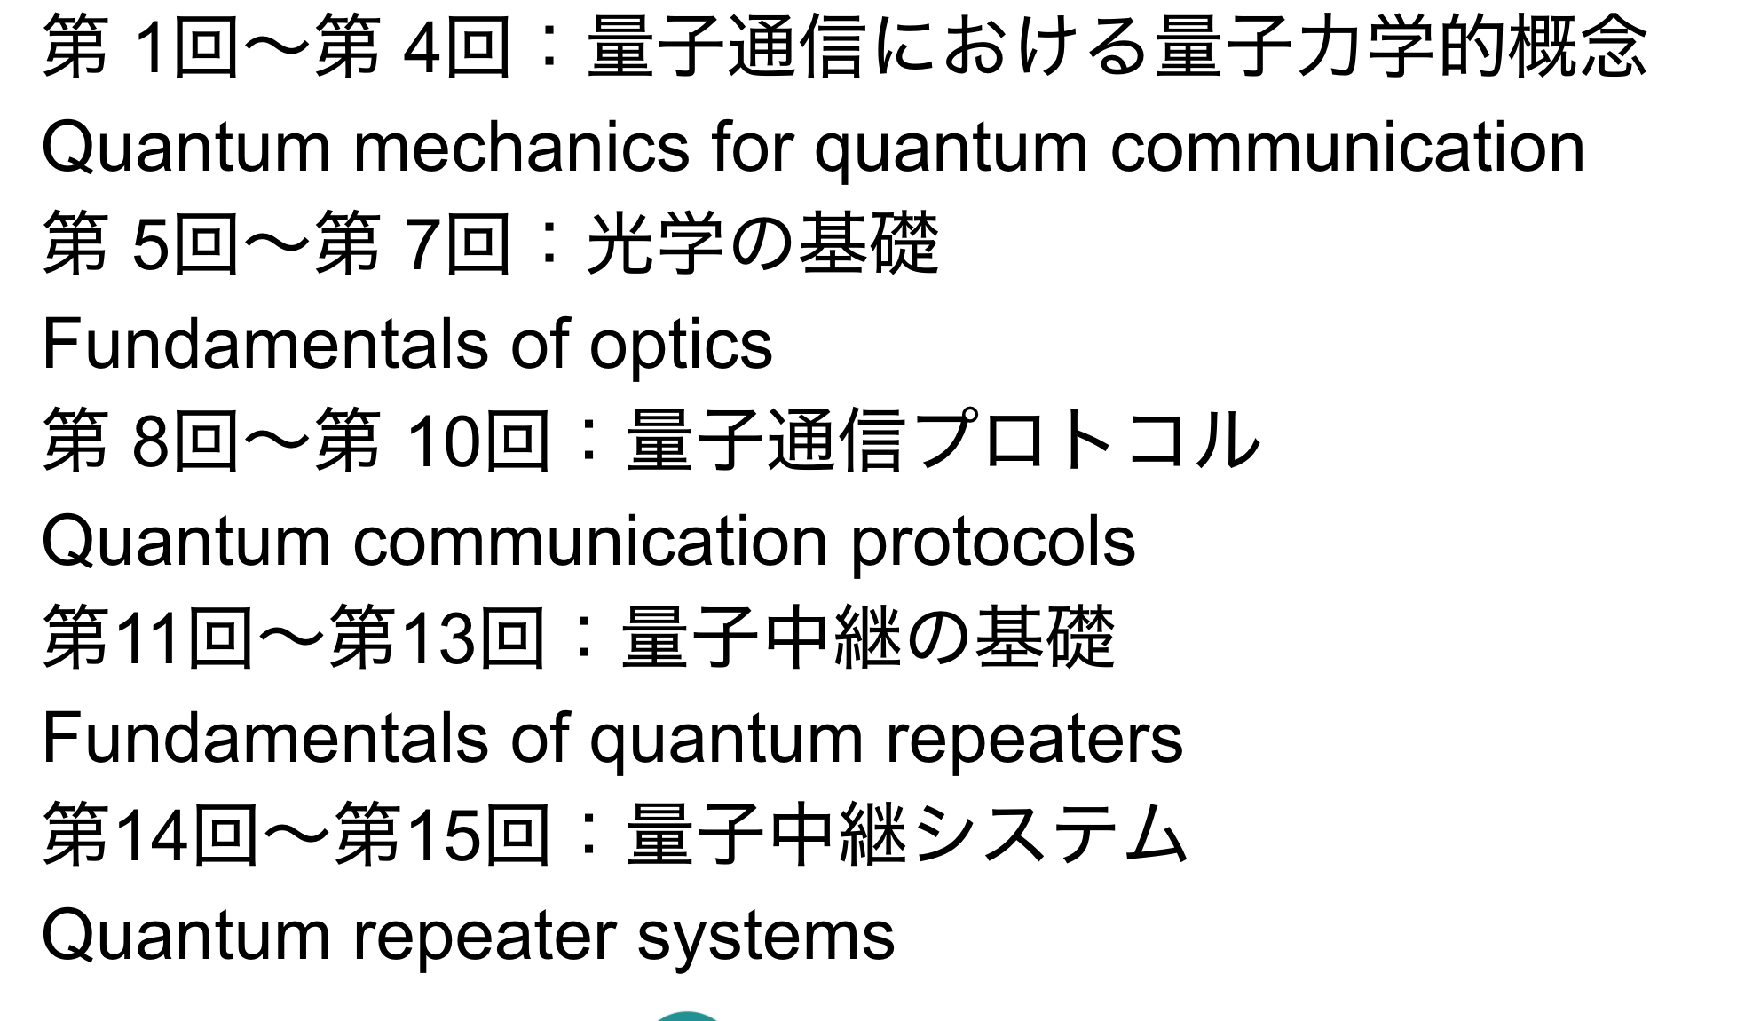
\includegraphics[width=0.8\textwidth]{lesson1/module_overview.pdf}
%     \label{fig:1-31}
%     \begin{center}
%         \caption{Module overview.}
%     \end{center}
% \end{figure}

% insert pre-requisities slide 
% \begin{figure}[H]
%     \centering
%     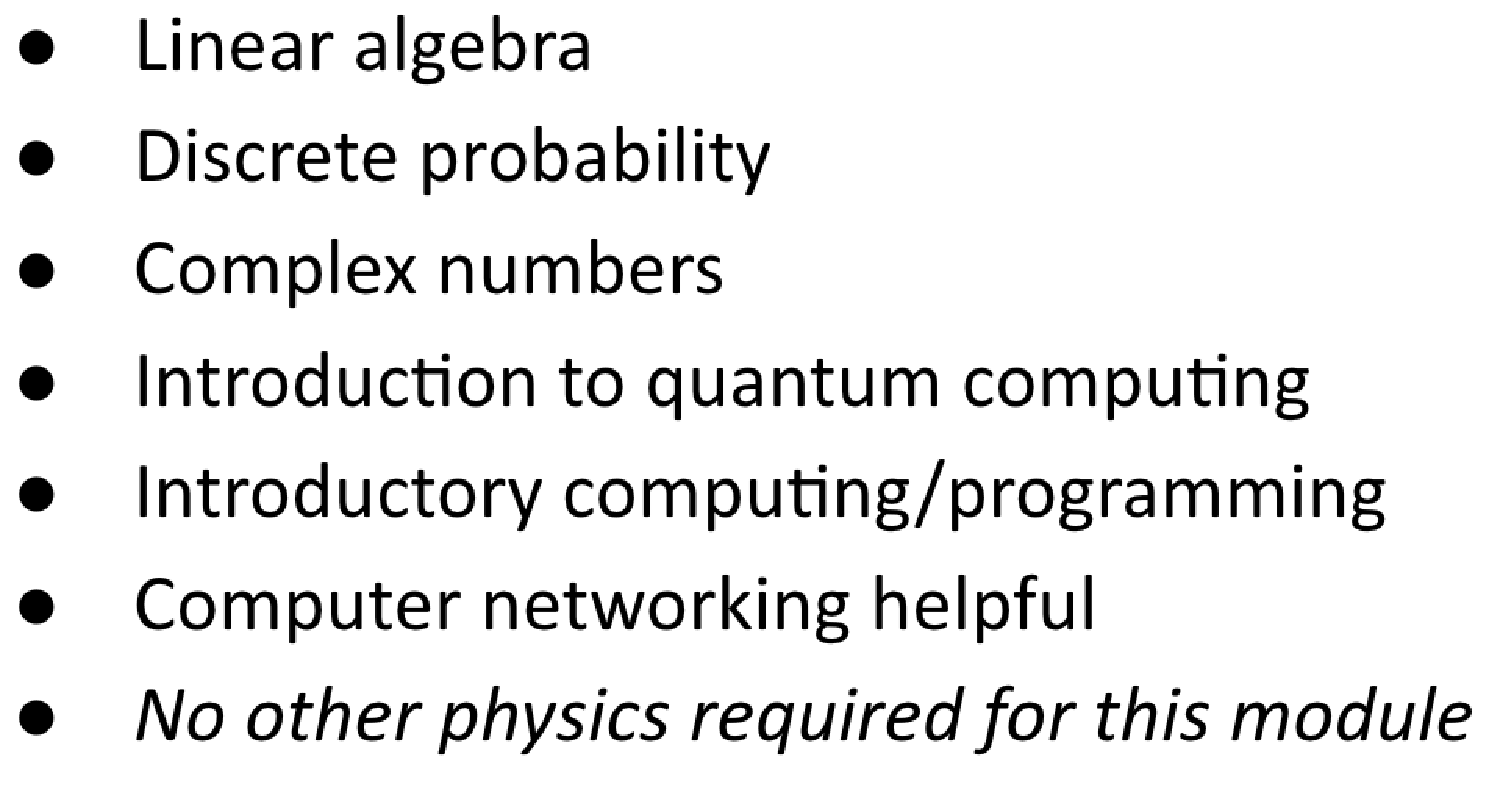
\includegraphics[width=0.8\textwidth]{lesson1/prereqs.pdf}
%     \label{fig:1-32}
%     \begin{center}
%         \caption{Prerequisites.}
%     \end{center}
% \end{figure}

% Rod videos pic
% \begin{figure}[H]
%     \centering
%     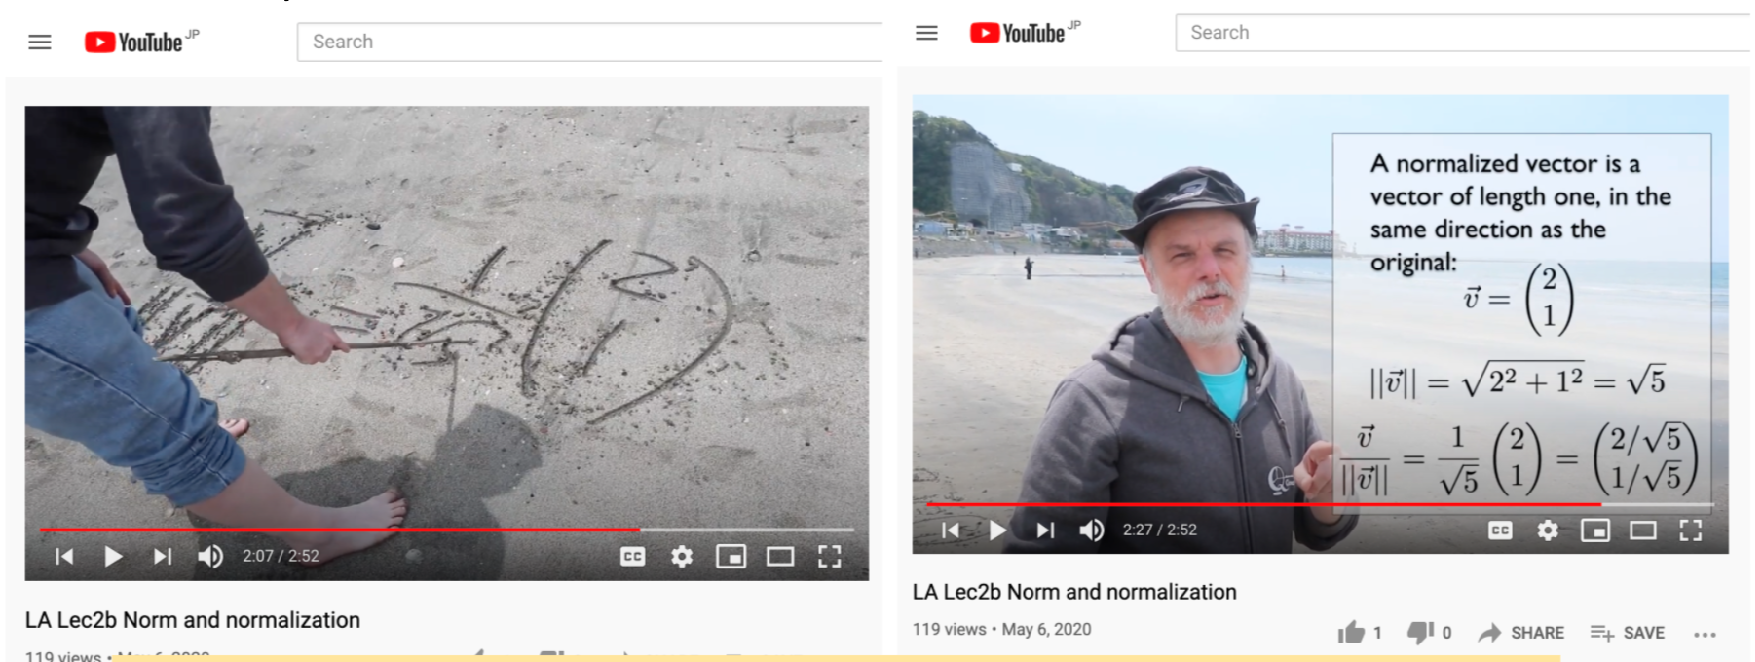
\includegraphics[width=1.1\textwidth]{lesson1/lin_alg_vids.pdf}
%     \label{fig:1-33}
%     \begin{center}
%         \caption{Linear Algebra videos.}
%     \end{center}
% \end{figure}

% \url{http://www.youtube.com/playlist?list=PLibMrvP9xUbeWZ1pCKnbTn2FO-c1PqHZr}.

% \newpage
% \begin{exercises}
% \exer{For Hooker's data, Exercise 1.2, use the Box and Cox and Atkinson procedures to determine a appropriate transformation of PRES
% in the regression of PRES on TEMP. find $\hat\lambda$, $\tilde\lambda$,
% the score test, and the added variable plot for the score. 
% Summarize the results.}

% \subexer{The following data were collected in a study of the effect of dissolved sulfur
% on the surface tension of liquid copper (Baes and Killogg, 1953).}


% \blankline
% \begin{tabular}{r@{}lcc}
% \hline
% &&\multicolumn2c{$Y$= Decrease in Surface Tension}\\
% \multicolumn2c{$x$ = Weight \% sulfur}
% &\multicolumn2c{(dynes/cm), two Replicates}\\
% \hline
% 0.&034&301&316\\
% 0.&093&430&422\\
% 011.&30&593&586\\
% \hline
% \end{tabular}
% \blankline

% \subexer{Find the transformations of $X$ and $Y$ sot that in the transformed scale 
% the regression is linear.}

% \subexer{Assuming that $X$ is transformed to $\ln(X)$, which choice of $Y$ gives 
% better results,
% $Y$ or $\ln(Y)$? (Sclove, 1972).}

% \sidebysidesubsubexer{In the case of $\Delta_1$?}{In the case of $\Delta_2$?}

% \exer{Examine the Longley data, Problem 3.3, for applicability of assumptions of the
% linear model.}

% \sidebysidesubexer{In the case of $\Gamma_1$?}{In the case of $\Gamma_2$?}
% \[
%     t= \frac{5}{256}\, \frac{c^5}{G^3}\,
%     \frac{r^4}{(m_1m_2)(m_1+m_2)}.  
% \]

% \end{exercises}

